\documentclass[english,master]{swsLeipzig}
% When you change the language, pdflatex may halt on recompilation.
% Just hit enter to continue and recompile again. This should fix it.

%
% Values
% ------
% \ThesisSetTitle{RAGBench - A Benchmark Framework for Retrieval-Augmented Generation Systems}
\ThesisSetTitle{RAGBench - Torwards Reconfigurable RAG Experimenation Without Overfitting}
\ThesisSetKeywords{RAG, benchmarking} % only for PDF meta attributes

\ThesisSetAuthor{Jan Albrecht}
\ThesisSetStudentNumber{3772326}
\ThesisSetDateOfBirth{17}{2}{1995}
\ThesisSetPlaceOfBirth{Freital}

\ThesisSetSupervisors{Prof.\ Dr.\ Norbert Siegmund,Prof.\ Dr.\ Unknown Yet}

\ThesisSetSubmissionDate{31}{1}{2025}

%
% Suggested Packages
% ------------------
\usepackage[sort&compress]{natbib}
%   Allows citing in different ways (e.g., only the authors if you use the
%   citation again within a short time).

% Let us get started by citing \citet{manning:1999}!
% So what did \citeauthor{manning:1999} do in \citeyear{manning:1999}?
% Good question!
\usepackage{multirow}

\usepackage{minted}


%
\usepackage{booktabs}
%    For tables ``looking the right way''.
%
%\usepackage{tabularx}
%    Enables tables with columns that automatically fill the page width.
%
%\usepackage[ruled,algochapter]{algorithm2e}
%    A package for pseudo code algorithms.
%
%\usepackage{amsmath}
%    For tabular-style formatting of mathematical environments.
%

%
% Commenting (by your supervisor)
% -------------------------------
\usepackage{xcolor}
\usepackage{soul}

% Graphical packages
\usepackage{graphicx}
\newcommand{\bscom}[2]{%
  % #1 Original text.
  % #2 Replacement text.
    \st{\scriptsize\,#1}{\color{blue}\scriptsize\,#2}%
  }
  
  \newcommand{\boldred}[1]{\textbf{\textcolor{red}{#1}}}
% Create links in the pdf document
% Hyperref has some incompatibilities with other packages
% Some other packages must be loaded before, some after hyperref
% Additional options to the hyperref package can be provided in the braces []
\usehyperref[backref] % This will add back references in the bibliography

\begin{document}
\begin{frontmatter}
  \begin{abstract}
    A short summary.
  \end{abstract}

  \tableofcontents

  %\chapter*{Acknowledgements} % optional
  %I thank the authors of the swsLeipzig template for their excellent work!

  %\listoffigures % optional

  %\listoftables % optional

  %\listofalgorithms % optional
  %    requires package algorithm2e

  % optional: list of symbols/notation (e.g., using the nomencl package)
\end{frontmatter}

\chapter{Introduction}\label{chap:introduction}
The year 2017 can be stated as the beginning of the interesting journey of artificial intelligent language models. With the publication of "Attention is all you need" from Vaswani \cite{vaswani2023attentionneed} the rapid development of language models and later large language models (LLMs) took off.

Today there is a variety of real world products that are using this technology, such as content generators like ChatGPT \cite{OpenAI_2022} or Claude \cite{Anthropic_2023}, translators like DeepL \cite{DeepL_SE} and Coding Assistants like Github Copilot \cite{Friedman_2022}. The list can be expanded with technologies like sentiment analysis, question answering systems, market research or education systems. Open-source models are available for each of these technologies, providing strong alternatives to proprietary services.

The remarkable capacity of large language models has led to wide acceptance in society. However LLMs have fundamental problems that cannot be solved with more training or larger models. Training models frequently is expensive, so daily training isn't feasible. Therefore every new information such as elections, weather or sport results that occurred between the last training and the user prompt are unknown to the model. On top of that, models can only be trained on available data. Private information of users that might be relevant for the prompt are not considered in the generation process. LLMs struggle also with long-tail information, which occurs rarely in the training data \cite{Kandpal.15.11.2022}.

When information is missing or underrepresented, outputs will deviate from user inputs, repeat previous outputs or may be made up by the LLM \cite{Zhang.03.09.2023}. This technology is already used in many sectors with billions of customers such as marketing, retail and eCommerce, education, healthcare, finance and law and media. It is crucial to develop systems that are as correct as possible.

The solution to potential missing information in training is to provide all necessary information to the LLM beforehand within the prompt, so that the generator just has to construct a coherent text for the user. This can be achieved with so-called Retrieval-Augmented Generation Systems (RAGs), where the raw user prompt is used to retrieve relevant data from a database that gets summarised and inserted into the prompt for the generator. This method overcomes many of the challenges LLMs face. Data can be accessed from private and up-to-date sources. The frequency of information occurrences no longer matters as long as the database includes it for retrieval. For having recent information, it is no longer required to train the underlying model.
% cite original RAG Paper
% cite paper that shows the advantages of RAG

However, the adoption of RAG systems introduces significant overhead and complexity. The system requires additional steps between the prompt request and output. Most of those steps can not be parallelized. That results in longer inference times and also leads to the more resource intensive system. Next to the increasing infrastructure costs, developing and maintaining a RAG is more time consuming than developing a LLM, because the LLM is a part of the larger system. RAGs are not by default significantly better systems than pure LLMs as Simon \cite{Simon.10112024} showed. These complex systems are highly sensitive to small configuration changes.

Therefore there is an important question to be asked: 
\begin{quotation}
    "Is an advanced RAG system necessary for your use case, or is a standalone LLM sufficient?"
\end{quotation}
\begin{quotation}
    "Is your RAG the best one for your specific use-case?"
\end{quotation}

The answers to these questions are hard to find, because you have to implement a RAG, to test it on your problem and your data. The scientific landscape of Retrieval-Augmented Generation Systems is a vast community with rapid development. Staying up-to-date with that research topic is time consuming for companies and research departments. 

The implementation of the RAG is just one part of the decision process. It is difficult to evaluate LLMs and all systems that are based on that technology, because outputs are not deterministic and such models are like a black-box. It is not obvious why the model responds with a certain output. Another problem is that there is a whole set of potential correct answers, because text-based outputs can have many forms. Lets consider following example:\\

Question: \textit{Is the evaluation process of LLMs an easy task?}\\
Answer 1: \textit{The evaluation process of LLMs is not an easy task.}\\
Answer 2: \textit{No, the evaluation process is a difficult task.}\\[6pt]

Both answers are correct, but which metric must be used to measure this outcome? 

The Evaluation of RAGs is even harder, because it has the same problems next to its own ones. RAGs are complex and is composed of many parts. Each part can lead to errors and therefore all components of the systems need to be evaluated next to an end-to-end evaluation of the whole system as Salemi \cite{Salemi.2024} and Yu \cite{Yu.2024} showed.

There are companies and research groups that successfully solved parts of this problem with developing tools, frameworks and libraries such as AutoRAG \cite{AutoRAG}, Llama-Index \cite{Liu_LlamaIndex_2022}, LangChain \cite{Chase_LangChain_2022}, RaLLe \cite{ralle}, FlashRAG \cite{FlashRAG}, RAGLAB \cite{zhang-etal-2024-raglab}, Haystack \cite{Pietsch_Haystack_the_end-to-end_2019} and FastRAG \cite{Izsak_fastRAG_Efficient_Retrieval_2023}. While an in-depth analysis will follow later in this thesis, it can be stated that all of those tools and frameworks are focussed on developing RAG-Variants, make them production-ready or evaluating them for performance, ignoring the fact that RAGs must be measured for hardware metrics like latency, inference time and CPU usage to determine if the benefits in performance compensate the disadvantages. Additional to this, Simon \cite{Simon.10112024} showed there is lack of external validity in the development of RAGs, because the iterative reconfiguration of those systems that leads to the best performance is a hyperparameter tuning process that overfits the model to the tested data and therefore requires a dataset split with a validation dataset and a holdout test dataset, which is only used to estimate the generalization error.

With this master thesis, we will make two contributions to the scientific landscape of RAGs: (i) A novel benchmarking framework, RAGBench, following the systematic blueprint shown by Simon \cite{Simon.10112024} and evaluating hardware metrics alongside SOTA performance evaluations, (ii) A practical demonstration of RAGBench through an experiment on the software engineering task of configuration validation. For (i), the framework will extend Haystack \cite{Pietsch_Haystack_the_end-to-end_2019} next to the FastRAG library \cite{Izsak_fastRAG_Efficient_Retrieval_2023}. Haystack is an open-source framework for LLMs, RAGs and SOTA search systems. FastRAG builds upon Haystack and adds special RAG architectures. 

The primary results of this work indicate that while RAG systems offer a powerful approach to overcoming LLM limitations, their effective implementation is non-trivial. The development of RAGBench highlighted the critical necessity of incorporating rigorous machine learning practices, such as a strict validation-test split, into RAG evaluation to mitigate overfitting. Furthermore, the application of RAGBench to software configuration validation revealed that retrieval quality is often the predominant bottleneck, and complex RAG architectures do not automatically surpass well-prompted standalone LLMs without careful, task-specific optimization of the retrieval components. Our experiments achieved a competitive F1-score of 0.776 for configuration validation using a standalone model with a Ciri-like few-shot setup, underscoring the importance of robust baselines.

This thesis concludes that a systematic and holistic benchmarking approach, as facilitated by RAGBench, is indispensable for advancing RAG technology. It enables data-driven decisions, helping to determine if a RAG system is truly necessary and how to best configure it for a specific use-case, moving beyond ad-hoc tuning towards more principled and reliable RAG solutions.

This thesis is structured as follows:
Chapter \ref{chap:background} provides an overview of the foundational concepts, including Large Language Models, text retrieval techniques, and the architecture of Retrieval-Augmented Generation systems.
Chapter \ref{chap:relwork} discusses existing research and tools related to RAG evaluation and benchmarking.
Chapter \ref{chap:design} details the design and methodology of the RAGBench framework, emphasizing its core principles for achieving generalizable and reproducible RAG experiments.
Chapter \ref{chap:Experiment} presents a practical application of RAGBench, detailing an experiment focused on using RAG for software configuration validation, and analyzes the obtained results.
Finally, Chapter \ref{chap:Conclusion} summarizes the contributions of this thesis and discusses the implications of RAGBench for future research and development in the field of retrieval-augmented generation.


\chapter{Background}\label{chap:background}


\section{Large Language Models}\label{sec:llm}
LLMs are deep neural network models trained on large corpora of text data. They are predominantly based on the Transformer architecture \cite{Wolf.09.10.2019}. Understanding Large Language Models and their hyperparameters like temperature or top-p is crucial for the development of RAG applications. Below, we explain the Transformer architecture and its main components.

\subsection{Transformer Architecture}
There are many well-known models based on the Transformer architecture, such as BERT, GPT-3.5, LLaMA, and others \cite{Yin.2024}. The Transformer architecture was introduced by Vaswani et al. in 2017. It's based on the self-attention mechanism, which allows the model to weigh the importance of each word in a sentence. The architecture has been shown to outperform other architectures in various NLP tasks.

% include graphic of Transformer architecture
\begin{figure}[!ht]
    \centering
    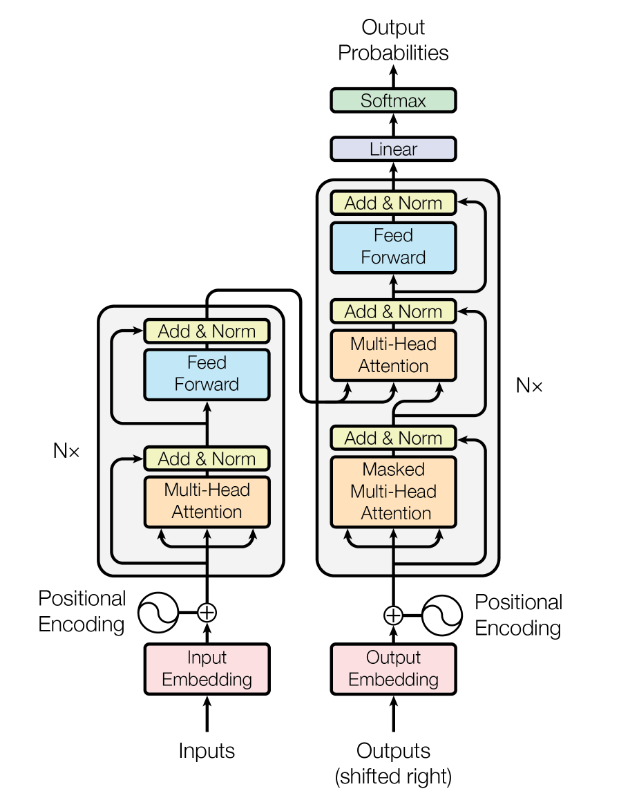
\includegraphics[width=0.6\textwidth]{images/transformers_architecture.png}
    \caption{Transformer Architecture with encoder (left) and decoder (right), Source: Vaswani \cite{vaswani2023attentionneed}}
    \label{fig:transformer_architecture}
\end{figure}

Figure \ref{fig:transformer_architecture} illustrates the Transformer architecture. Both encoder and decoder can be standalone models. Text must be tokenized through a dictionary to have a fixed size and frozen vocabulary.
The encoder embeds a sequence of tokens and passes them to the the positional encoding layer to preserve information for token position. Subsequently, it passes through multiple layers of multi-head self-attention and feed-forward neural network blocks. Attention heads compute token relevance via scaled dot-product
$softmax(QK^T/\sqrt{d_k})V$ where Q,K,V are learned projections. The outputs of the encoder is a real-valued numberical vector and can be passed to the decoder.
The decoder embeds an empty or predefined sequence. It gets passed to several layers of masked and non-masked multi-head self-attention, plus a feed forward neural network blocks. The mask ensures the decoder can only use preceding tokens. The output probabilities forecast the next token in sequence. Therefore prior decoder outputs can be used to autoregressively generate sequences of tokens.

% \paragraph{Encoder}

% The encoder transforms the sequences in a list of tokens and passes them to the input embedding layer and to the the positional encoding layer. Subsequently, it passes through multiple layers of multi-head self-attention and feed-forward neural network blocks. The outputs of the encoder is passed to the decoder, if the architecture is an encoder-decoder architecture. Encoders can also stand alone for tasks like text and code classification. (\citet{Hou.8212023})

% \paragraph{Decoder}

% In the encoder-decoder architecture the decoder begins with an initial output sequence or an empty sequence. The output sequence is passed to the output embedding layer and to the positional encoding layer. After that it gets passed to several layers of masked and non-masked multi-head self-attention, plus a feed forward neural network blocks. The outputs of the decoder is passed to the output layer, which is a linear layer followed by a softmax function. The output layer predicts the next token in the output sequence. The output sequence is passed to the decoder again, so that the model can predict the next token based on the previous tokens. This process is called autoregressive generation.
% The decoder can also stand-alone for autoregressive tasks like code completion, text to code generation, debugging, etc. as shown in \citet{Hou.8212023}.

% \paragraph{Input Embedding}
% Depending on the model, the input and output sequences are tokenized into subwords, words or characters. The input embedding layer converts tokenized sequences into dense vector representations. The input embedding layer is trained along with the rest of the model. The output of the input embedding layer is passed to the positional encoding layer. The positional encoding layer adds information about the position of each token in the input sequence, so that the model can distinguish between words with the same token but different positions. Positional encodings are combined with input embeddings before being fed into the encoder. The output embedding is equivalent to the input embedding, but it is used to convert the output tokens into a dense vector representation. The output embedding is used in the decoder part of the Transformer architecture.

% \paragraph{Multi-Head Self-Attention Block}

% Both in the encoder and in the decoder, a block consists of several multi-head self-attention layers followed by a feed-forward neural network layer. The multi-head self-attention layer is the main component of the Transformer architecture. It allows the model to weigh the importance of each token in the input sequence for each other token. The multi-head self-attention layer consists of multiple heads. Each head consists of a Query, Key and Value matrix, which are used to calculate the attention scores between the input tokens. The attention scores are used to weigh the importance of each token in the input sequence for each other token. The attention mechanism is mathematically defined as:

% $$Attention(Q,K, V) = softmax(\frac{QK^T}{\sqrt{d_k}})V$$

% Query (Q), Key (K) and Value (V) are matrices of the input tokens. This mechanism is based on common retrieval. Query can be seen as the search query, Key as the potential candidates and Value as the retrieved information.

% All matrices are learned during training. Query and Key are used to calculate the attention scores. The division by $\sqrt{d_k}$ is used to stabilize the gradients during training. The softmax function is used to normalize the attention scores. For the decoder part with the masked multi-head self-attention, the attention scores are masked with $-\infty$ for every token after the current calculated one right before the softmax, so that the model can only attend to previous tokens in the output sequence and the next predicted token is based only on the previous tokens. All attention heads are concatenated, passed through a linear layer, which is finally followed by a layer normalization to stabilize the gradients during training. 

% \paragraph{Putting it all together}
% After the input sequence is passed through the encoder, the output sequence is passed through the decoder. The decoder uses the encoder output as additional input and autoregressively predicts the next token in the output sequence. The output sequence is passed to the output layer, which is a linear layer followed by a softmax function. The output layer predicts the next token in the output sequence. The output sequence is passed to the decoder again, so that the model can predict the next token based on the previous tokens. This process is called autoregressive generation.

% There are several ways to predict the next token within the output layer. The most straightforward way is to predict the token with the highest probability. This is called greedy decoding. Another way is to sample the next token from the probability distribution. This is called sampling. There are also other ways to predict the next token, such as beam search, nucleus sampling, top-k sampling, top-p sampling, etc. These methods are used to improve the performance of the model. In the following the most important tuning parameters for LLMs are explained.

\subsection{Tuning Parameters}

There are several tuning parameters that can be used to improve the performance of LLMs. Some of the most important tuning parameters are:

\paragraph{Temperature}
The temperature parameter is used to control the randomness of the generated text. A high temperature value leads to more randomness, while a low temperature value leads to less randomness. The temperature parameter T modifies the softmax function as follows:

%include graphic
\begin{figure}[h!]
    \centering
    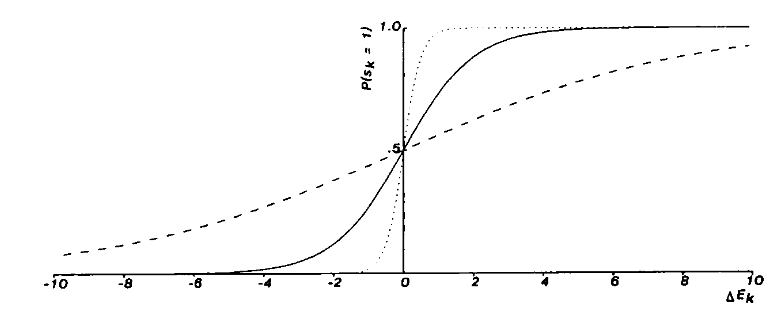
\includegraphics[width=0.6\textwidth]{images/temperature.png}
    \caption{The softmax function with different temperature values, T=1.0 (solid), T=4.0 (dashed), T=0.25 (dotted), Source: Ackey et al.\cite{ACKLEY.1985}}
    \label{fig:temperature}
\end{figure}

$$softmax: o(z)_i = \frac{e^{\beta z_i}}{\sum_{j=1}^K e^{\beta z_i}}$$

In figure \ref{fig:temperature} the softmax function is shown. A low temperature value leads to a peaky distribution, while a high temperature value leads to a more uniform distribution and therefore to more randomness.


% split paragraph in two parts
\paragraph{Top-K Sampling}
Top-K sampling \cite{Fan.13.05.2018} randomly selects from the top K tokens with the highest probability before applying the softmax function. Therefore the higher the K value, the more tokens are considered for sampling. Higher values increase output randomness. With Top-K equal to 1, the model behaves like greedy decoding.

\paragraph{Top-P Sampling}
The Top-P sampling \cite{Holtzman.22.04.2019} randomly selects from the smallest set of tokens whose cumulative probability exceeds the probability P. Therefore the higher the P value, the more tokens are considered for sampling. The outcomes gets more random. It is a generalization of Top-K sampling, where the number of tokens to sample from is not fixed.

\subsection{Prompting Techniques}
The Transformer architecture is not deterministic as shown in previous sections. Additionally LLMs have a high variance for its outputs too. The input prompt critically influences output quality. Therefore there are plenty of prompting techniques to stabilize desired outputs. Schulhoff created a taxonomy and recognized 58 LLM prompting techniques \cite{Schulhoff.06.06.2024}. We discuss four representative prompting techniques: Few-Shot, Zero-Shot, Chain-of-Thought (CoT), and Chain-of-Verification (CoVe). The list is not complete, but those are very commonly used and easy to implement.

\paragraph{Few-Shot vs. Zero-Shot}

\begin{figure}[h!]
    \centering
    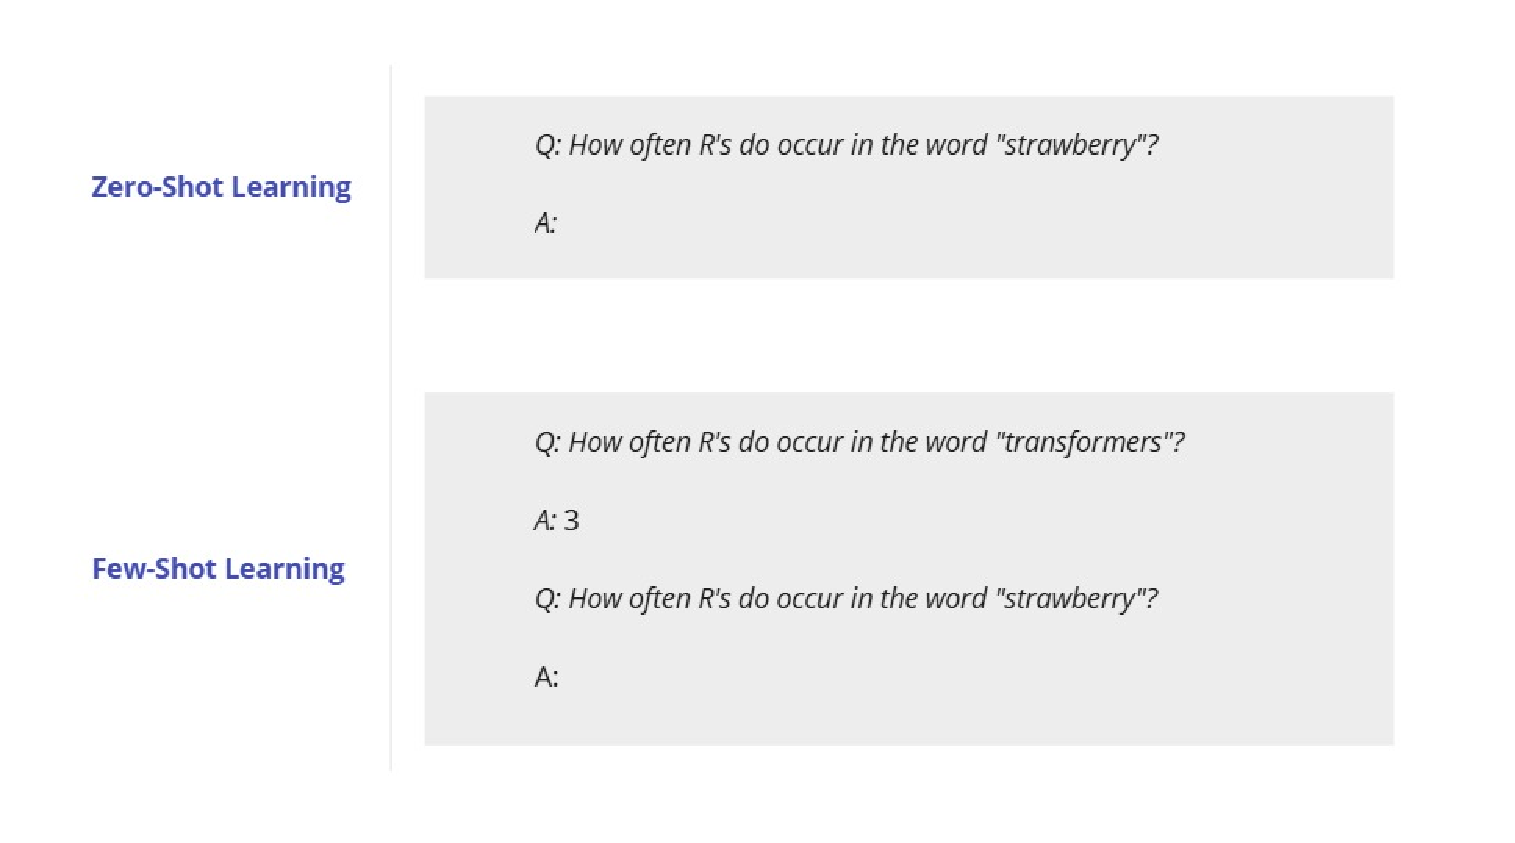
\includegraphics[width=\textwidth]{images/FewShot vs ZeroSHot.pdf}
    \caption{An example with a difficult query, that many LLM struggle, first without example (Zero-Shot) and below with one example (Few-Shot).}
    \label{fig:FewZeroShot}
\end{figure}


Few-Short prompting is a form of In-Context Learning (ICL), in which the prompt has examples of similar tasks to show the model how a task should be done. Brown showed that large models can leverage examples for various tasks \cite{Brown.28.05.2020}. Zero-Shot prompting refers then to prompting without showing examples before the task. Even though Few-Shot prompting might increase performance of LLMs, it comes with increased costs, as there are more tokens to process. An example of those prompting methods can be seen in figure \ref{fig:FewZeroShot}.

\paragraph{Chain-of-Thought}

\begin{figure}[h!]
    \centering
    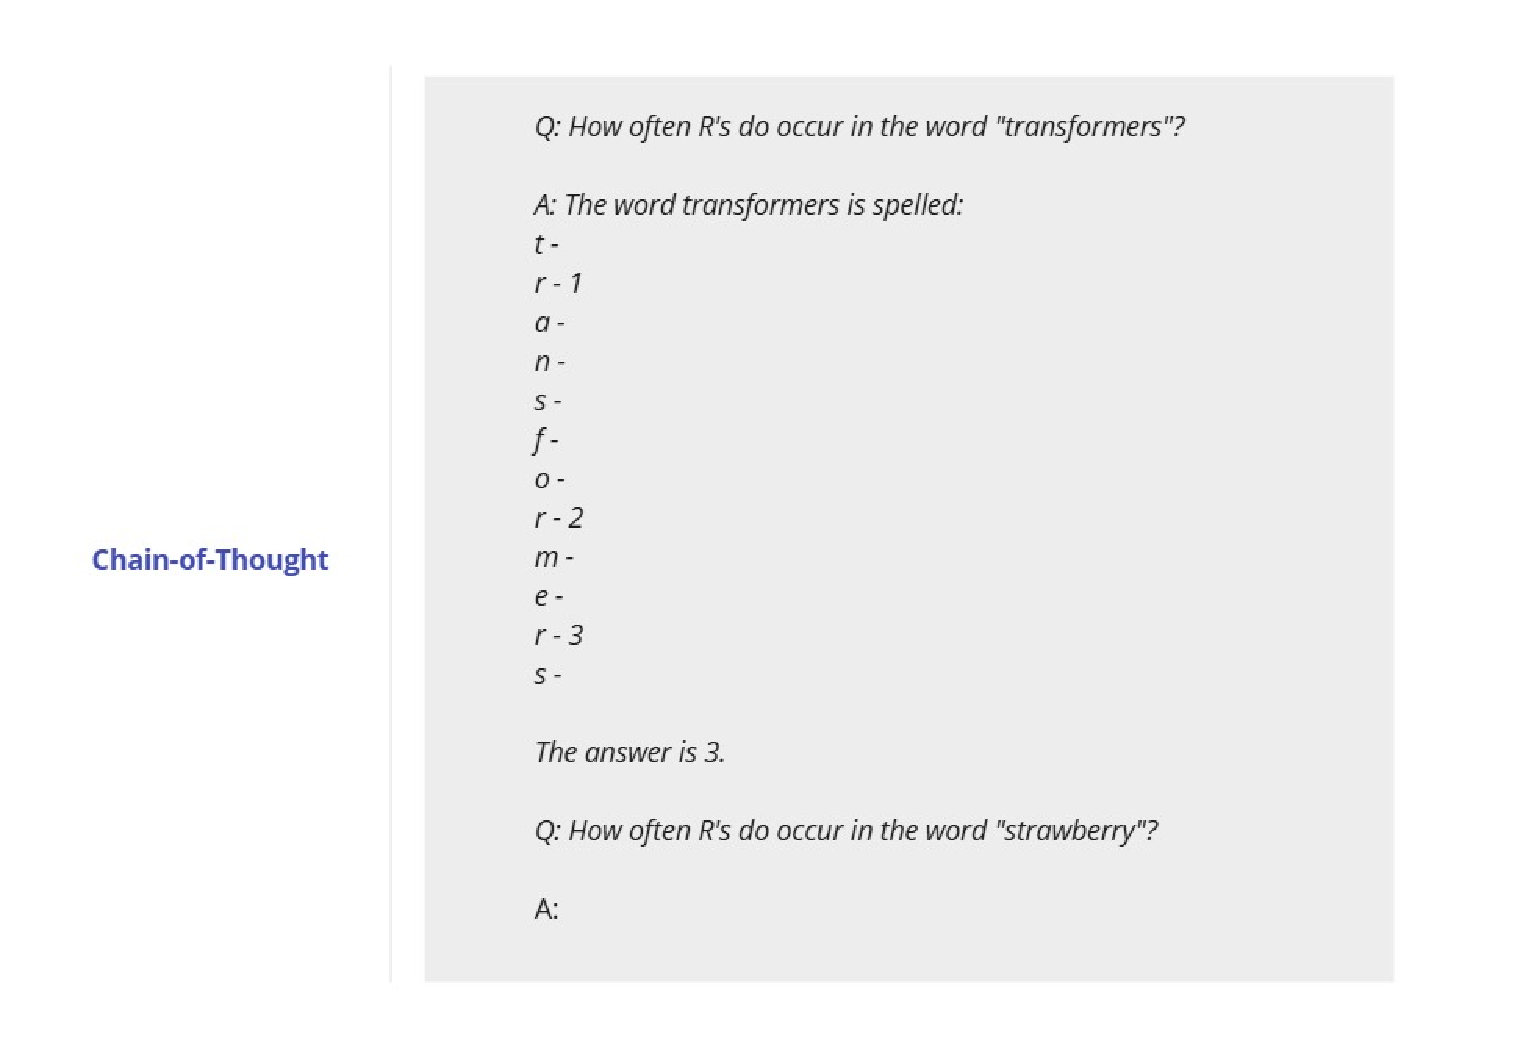
\includegraphics[width=\textwidth]{images/Chain-of-Thought.pdf}
    \caption{An Chain-of-Thought example with a difficult query, that many LLM struggle without prompting techniques}
    \label{fig:CoT}
\end{figure}


This method introduced by Wei leverages Few-Shot learning through simulating a written thought process in prior examples \cite{Wei.28.01.2022}. The LLM is therefore forced to take over this behaviour, which leads to more accurate outputs in reasoning and math problems. Schulhoff refers to it as the class of Thought Generation techniques \cite{Schulhoff.06.06.2024}. Figure \ref{fig:CoT} shows an example prompt.

\paragraph{Chain-of-Verification}


\section{Text Retrieval}\label{sec:retrieval}
%!TEX encoding = UTF-8 Unicode

There are several types of text retrieval for RAG systems. \citet{Zhao.29.02.2024} classified four different types of retrieval techniques regarding how the retrieved information are passed to the generation. In this thesis I will only focus on query-based retrievals as they are the most common and widely used retrieval techniques. The other three types are latent-representative-based retrieval, logit-based and speculative retrieval.

Another categorization of text retrieval can be done by the type of retrieval. There are three main types of retrieval: sparse retrieval, dense retrieval and hybrid retrieval. Sparse retrieval is based on traditional information retrieval techniques like TF-IDF or BM25. Dense retrieval is based on transformers models and hybrid retrieval combines both sparse and dense retrieval techniques. Following I  will describe those techniques in more detail.
\subsection{Sparse Retrieval}
\label{sec:sparse_retrieval}

\paragraph{TF-IDF}
\label{sec:tfidf}

TF as shown in \citet{Manning.2009} refers to the term frequency of a term $t$ in a document $d$. The inverse document frequency (IDF) is calculated as the logarithm of the total number of documents $N$ divided by the number of documents containing the term $t$. Therefore the IDF factor is low for terms that occur in all documents and high for distinguishing terms that occur in frequently in a low number of documents. The position of the words is ignored.

$$\textit{TF-IDF}(t, d, D) = \textit{TF}(t, d) \cdot \textit{IDF}(t, D) = \textit{TF}(t, d) \cdot \log\left(\frac{N}{\textit{DF}(t, D)}\right)
$$

\paragraph{BM25}
\label{sec:bm25}

\citet{Manning.2009} showed several versions of it. One simpler one is defined as following.


$$BM25(t, d, D) = IDF(t, D) \cdot \frac{(k_1 + 1) \cdot TF_{t, d}}{k_1((1-b)+b \cdot \frac{L_d}{L_{ave}}) + TF_{t, d}}$$


The BM25 score is an advanced version of the TF-IDF score with two free parameters $k_1$ and $b$. The parameter $k_1$ is a scaling factor to determine how relevant term frequency is. The parameter $b$ is for document length scaling, reducing scores of long documents.

\subsection{Dense Retrieval}
\label{sec:dense_retrieval}

Dense Passage Retrieval as shown in \citet{karpukhin2020densepassageretrievalopendomain} utilizes Bidirectional Encoder Representation from Transformers (BERT, \citet{devlin2019bertpretrainingdeepbidirectional}). BERT can be seen as the encoders part of an sequence-to-sequence transformers architecture. Therefore it can be used to encode the text passages used as contexts at the classification token [CLS]. The text is thus mapped into an d-dimensional real-valued space with the assumption that semnatic similar passages are close to each other in this space. The query is also encoded into this space and the similarity between the mapped query vector and each passage vector is calculated. The similarity is calculated by the dot product or other similarity functions. The top-k similar passages are then selected and used for the generation.

Nowadays there are highly specialized embedding models, that are benchmarked and listed on the Huggingface MTEB as described in \citet{muennighoff2022mteb}. Even though the MTEB leaderboard suggests a best-of-all embedding model, there is no such thing. Embedding models are language- and domain-sensitive as \citet{Gao.18.12.2023} points out. 

\subsection{Hybrid Retrieval}
\label{sec:hybrid_retrieval}

Both sparse retrieval techniques TF-IDF and BM25 are good for keyword specific searches, but perform poorly on a semantic comparison of documents and query. Encoders like BERT were trained for understanding languages and are thus good for a semantic understanding. Often it is not trivial to dertermine if a text retrieval needs a keyword-relevant sparse retrieval or dense retrieval considering semantics. 

Hybrid models calculate both dense retrieval and sparse retrieval scores and multiply it then with factor $\alpha$ and $1-\alpha$ respectively. An factor $\alpha=1$ results in using only dense retrieval. There is no universal performant value for $\alpha$. Therefore this is a hyperparamter tuning parameter that needs to get optimizied.



% \section{Vector Databases}\label{sec:vdbs}
% Storing high-dimensional vector data cannot be done efficiently with traditional databases. Vector databases (VDBs) specialize in efficiently searching for semantically similar entities within high-dimensional data. Especially for dense retrieval, similarity search is a highly complex topic. Given a query vector $v_1$, finding the nearest neighbor $v_{n}$ would require comparing $v_1$ with every vector in the dataset. Jing \cite{Jing.2024} notes this brute-force approach yields $O(dN+N$ $log$ $k)$ complexity, making it impractical for large-scale applications. Efficient alternatives to brute-force search constitute the key differentiating capability of modern vector database systems. To date, no comprehensive comparison of search latency across VDB providers exists to our knowledge. Pan \cite{Pan.2024} compared providers regarding features they offer and pointed out that cross-disciplinary comparisons of vector search algorithms and systems are scarce.

While numerous optimization techniques exist, this thesis focuses on two representative methods: We detail Product Quantization (PQ) and the Hierarchical Navigable Small World (HNSW) algorithm, a state-of-the-art approximate nearest neighbor (ANN) method—due to their widespread adoption and effectiveness. I refer to Jing \cite{Jing.2024} and Kukreja \cite{Kukreja.2023}, who explained many other techniques in great detail.

\paragraph{Hierarchical Navigable Small World (HNSW)}

\begin{figure}[h!]
    \centering
    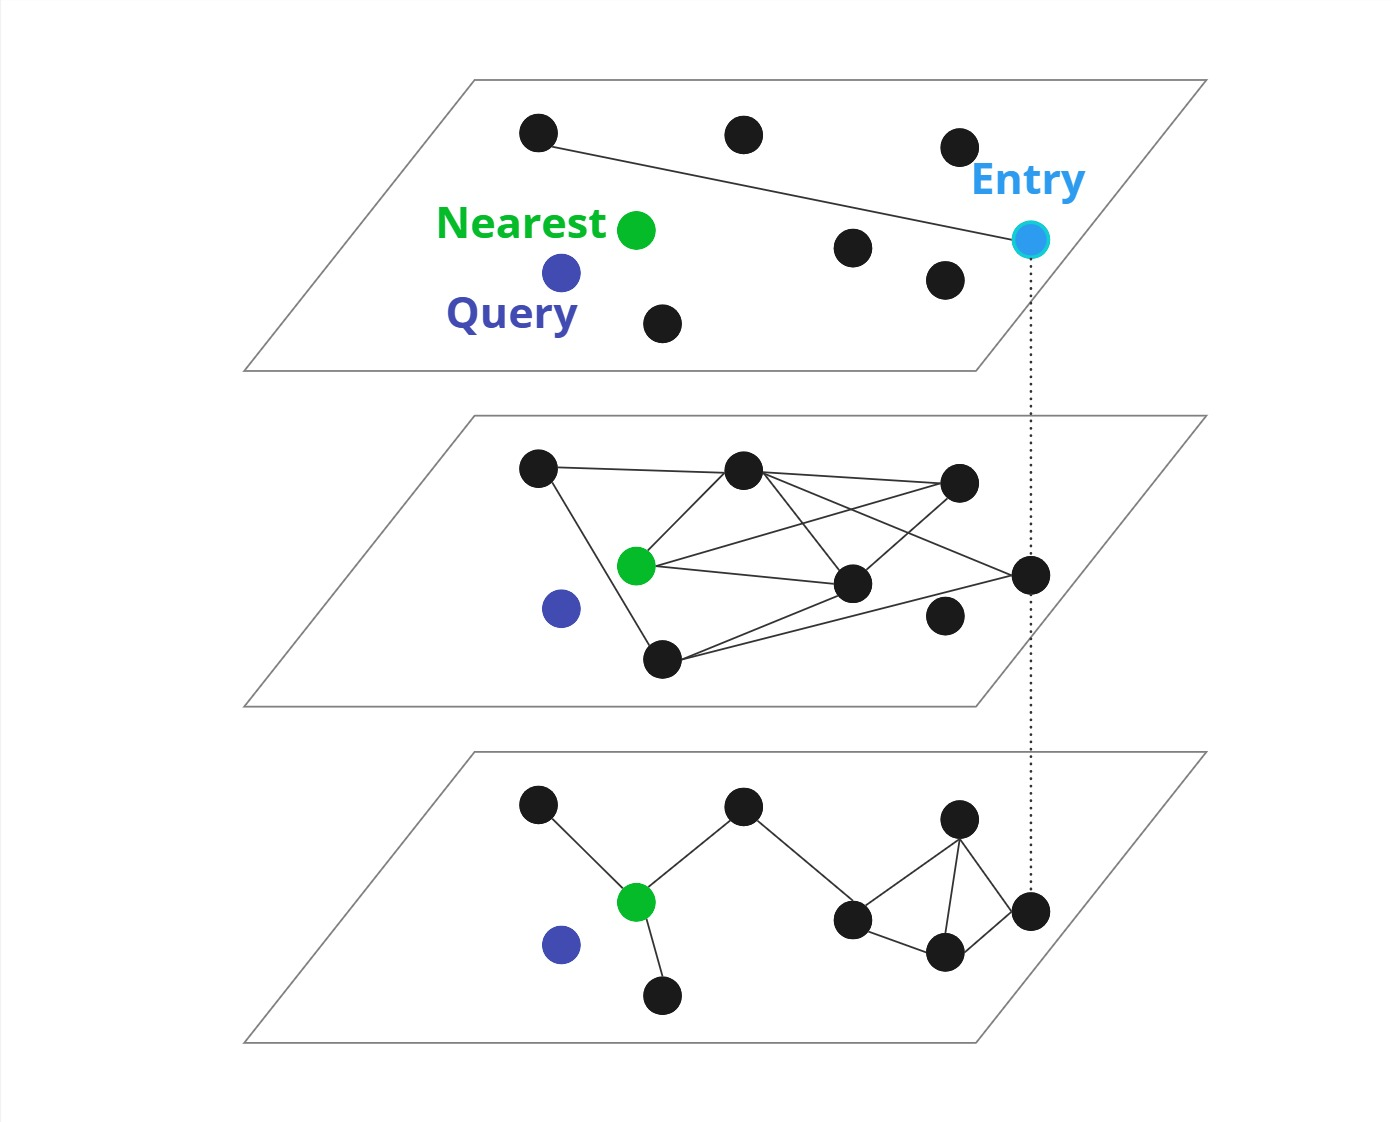
\includegraphics[width=\textwidth]{images/HNSW.jpg}
    \caption{HNSW algorithm visualized, highly inspired by \cite{Pinecone.22.01.2025}}
    \label{fig:HNSW}
\end{figure}

Approximate Nearest Neighbor is a term referencing all Nearest Neighbor algorithms that do not search for the most similar or closest point, but rather for a match that is close enough. One version of that is the HNSW algorithm, which was developed by \cite{Malkov.2014} and uses a skip-pattern invented by \cite{Pugh.1990}. The algorithm is visualized in figure \ref{fig:HNSW}. HNSW constructs a hierarchical graph where nodes connect via randomly sampled edges across multiple layers. Upper layers contain long-range connections, while lower layers progressively feature shorter, localized edges. The algorithm starts comparing on the top-level layer and if it reaches a local minimum, it continues on the next layer until it finds its local minimum on the bottom layer. While HNSW sacrifices guaranteed optimality, it achieves a favorable trade-off between recall and execution speed, as demonstrated by \cite{ErikBernhardsson.22.01.2025}.


\section{Retrieval-Augmented Generation Systems}\label{sec:rag}
Large language models (LLMs) exhibit fundamental limitations that cannot be fully resolved through training or prompt engineering. Gao \cite{Gao.18.12.2023} stated that LLMs have significant limitations in knowledge-intesive or domain-specific tasks. Insufficient domain-specific training data often results in erroneous outputs. For large language models this is called \textit{hallucinations} as defined in Huang \cite{Huang.2023}. In retrieval-augmented generation (RAG) systems, hallucinations refer to outputs unsupported by provided context. Rashkin \cite{Rashkin.} defined hallucinations as any information that is neither inferable from nor stated by an external document. In this thesis we will use the definition for RAG systems. 

Factual wrong output from an LLM can have several reasons. The required information to answer this question can be private, stored on a database that is not accessible during training. Additionally, the high cost of training/fine-tuning limits update frequency. This creates temporal gaps where post-training information remains unavailable. All those problems can be solved if the LLM is not used for the answer itself, but rather used for building a coherent text passage given a question and its answer. Then a database would store all relevant information and would be updated as frequent as required. During inference, the system retrieves relevant document chunks from the database to inform answer generation.

This concept is very successful as Shuster \cite{Shuster.} showed. This approach reduces factual errors while enhancing open-domain conversational performance. Yu \cite{Yu.2024} concluded that this improves the reliability and richnes of the produced content. Chen \cite{Chen.2024} identifies external knowledge integration as crucial for improving LLM accuracy and reliability.

There is a high variety in architectures and approaches for retrieval-augmented generation models. In this section, we will give an overview of the most common approaches and architectures and start with the most basic ones. The section will follow the definition of RAGs in Gao \cite{Gao.18.12.2023} with naive RAGs, advanced RAGs, a modular architecture, and special cases. 

\subsection{Naive RAGs}
\label{sec:naive_rags}
Naive RAGs represent the foundational implementation of retrieval-augmented generation. These systems concatenate retrieved context with user queries to guide LLM responses. Then the LLM is only used for generating a coherent answer. Therefore it is required to ingest relevant data for the given use case beforehand. The system then retrieves relevant chunks or documents of this data at inference time. 


\begin{figure}[h!]
    \centering
    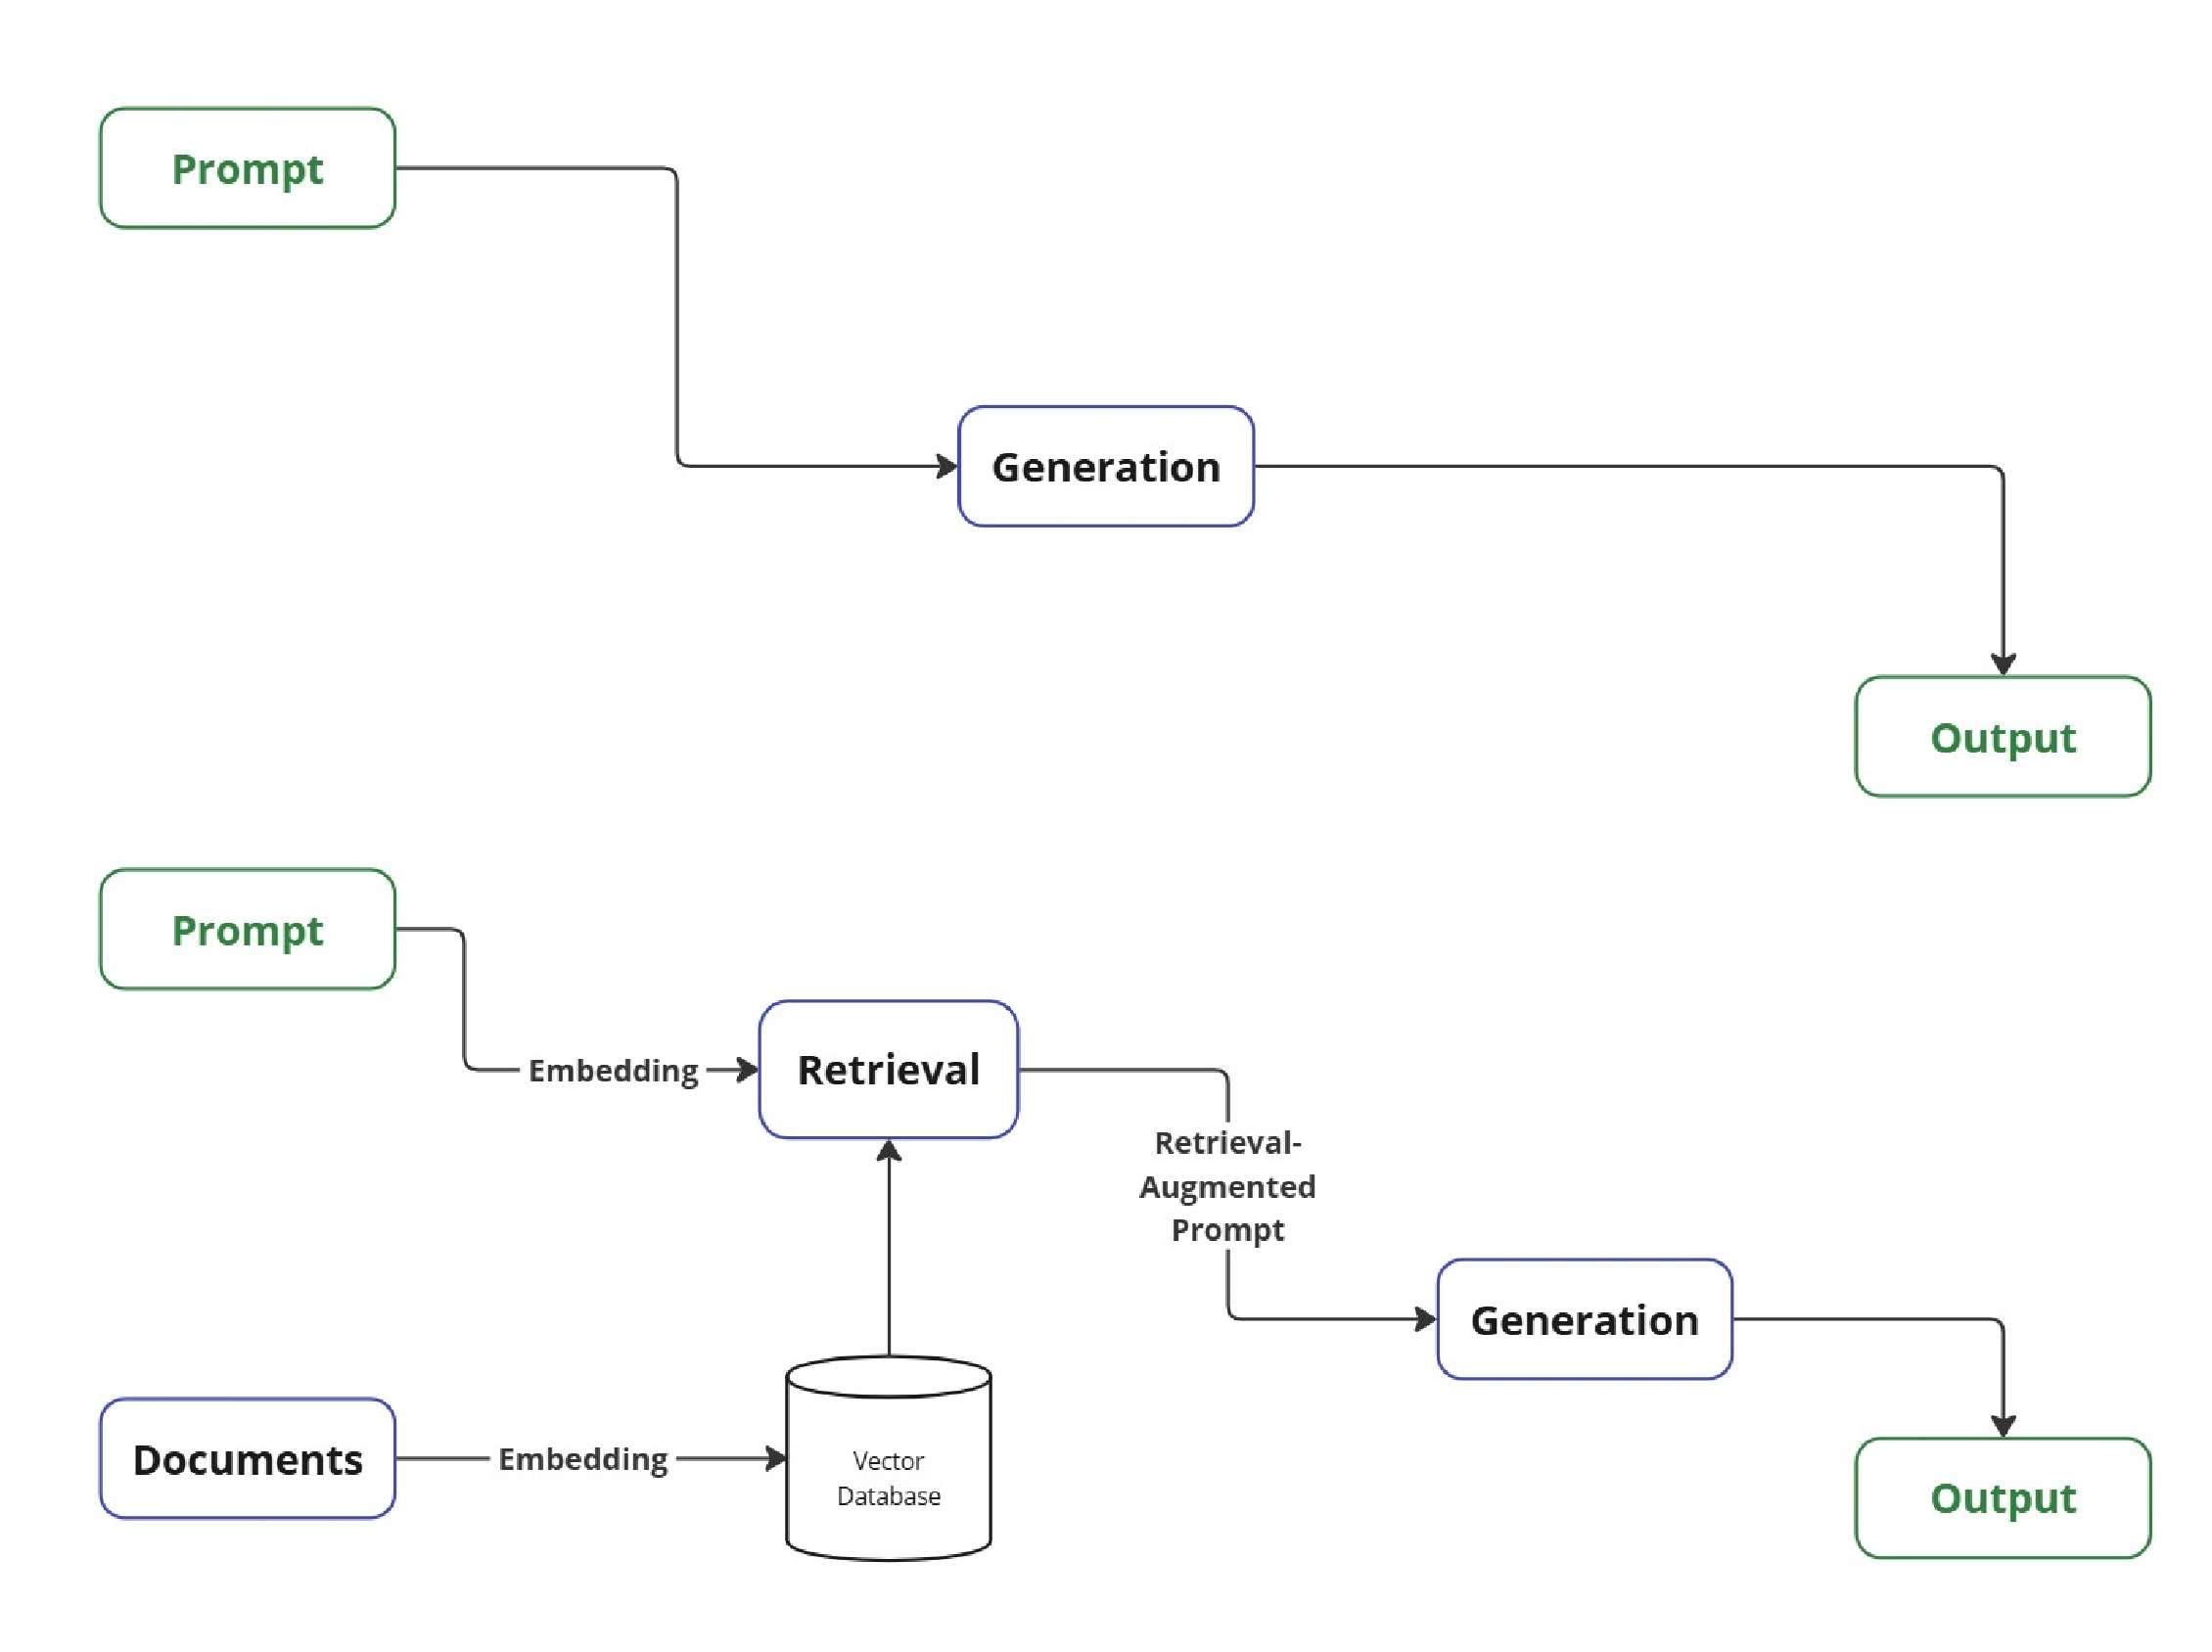
\includegraphics[width=\textwidth]{images/LLM-vs-RAG.pdf}
    \caption{Comparison of the process, above a standalone LLM that has a prompt and generate a response, below a minimalistic RAG system that performs on a given set of documents an embedding or indexing and searchs for the most similar documents for a given prompt at inference time. Both prompt and documents are used for the generation process.}
    \label{fig:naive_rag}
\end{figure}

This procedure can be seen in figure \ref{fig:naive_rag}. This generation phase is frequently termed the \textit{read} operation in literature. Gao \cite{Gao.18.12.2023} defines the naive RAG system as \textit{Retrieve-Read}. The retrieval can be done with sparse retrieval (TF-IDF, BM25), dense retrieval (DPR) or a hybrid version as showed in section \ref{retrieval}. 

\begin{figure}[h!]
    \centering
    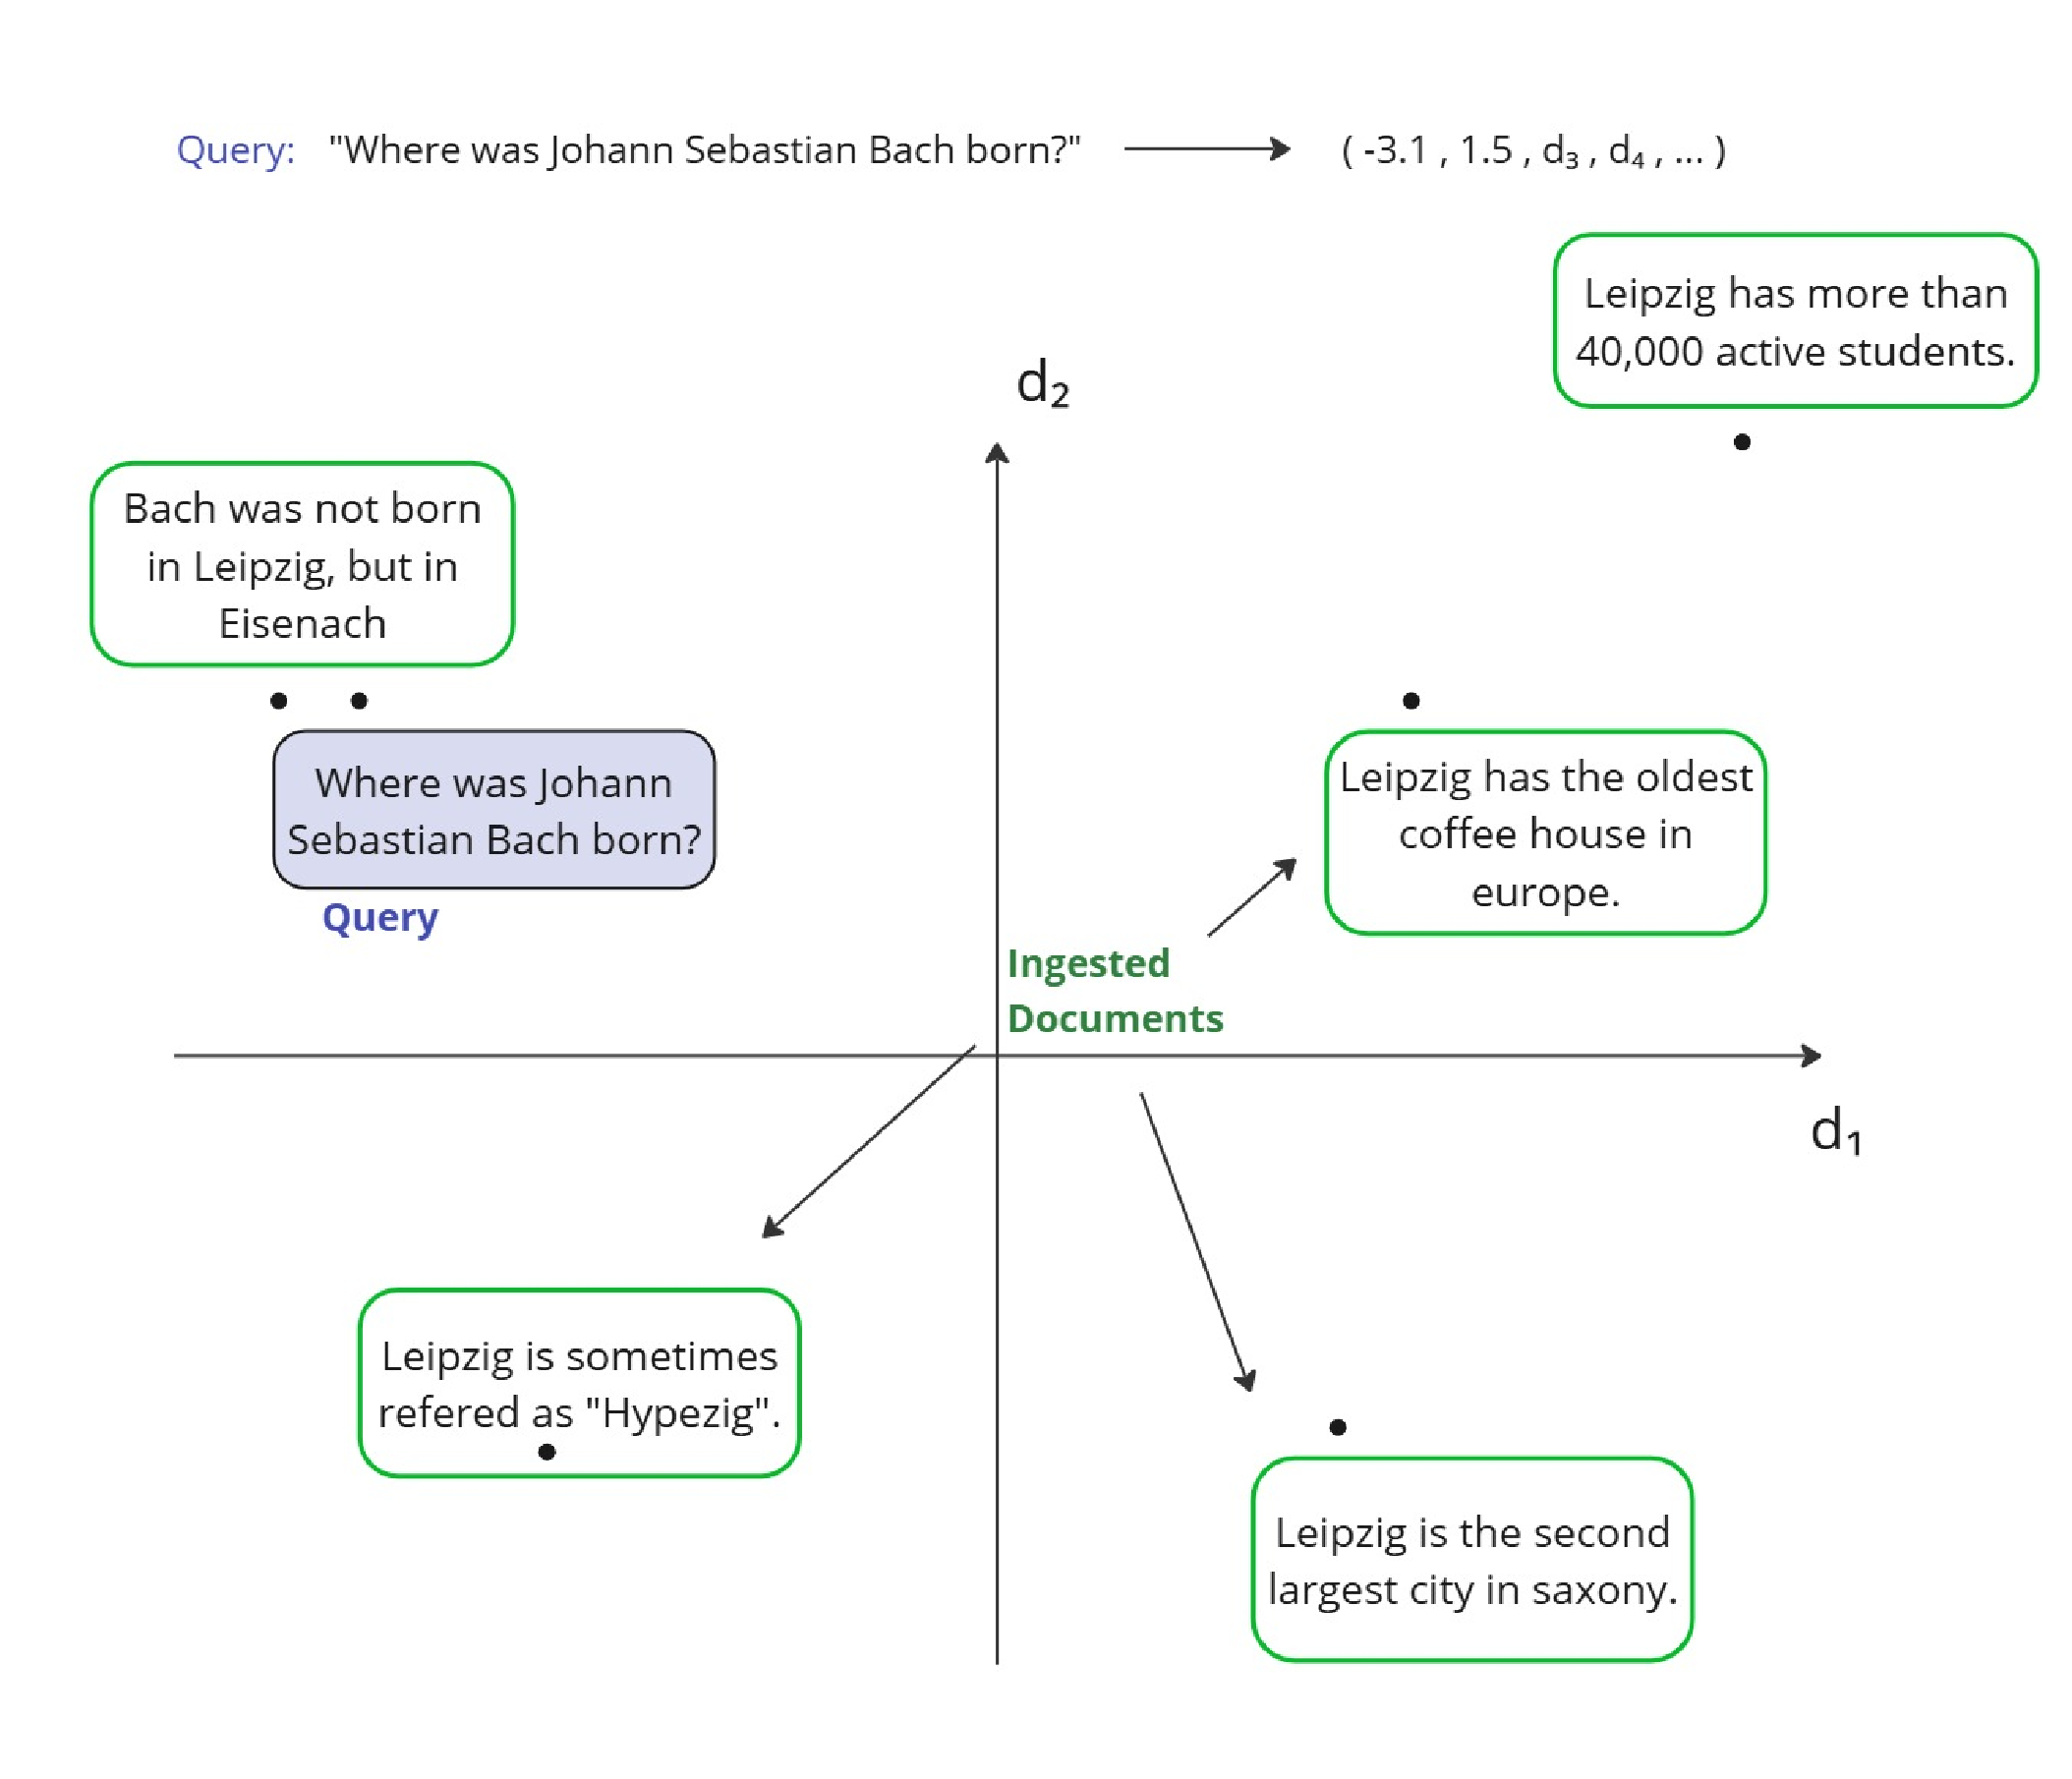
\includegraphics[width=\textwidth]{images/VectorDB.pdf}
    \caption{A vector space including mapped facts (documents) and a user query. The query and its correct answer have similar vectors}
    \label{fig:vectorDB}
\end{figure}


Before the system can be used, it is necessary to ingest data. The ingestion process includes preprocessing and selection of data, that users are likely to need for their questions or use cases. Therefore it is relevant to know the user base. It is not feasible nor efficient to ingest all availlable data. The preprocessing pipeline converts raw data into document chunks using methods detailed in Section \ref{sec:chunk}. As described in \ref{sec:dense_retrieval}, the chunks are then embedded into a d-dimensional real-valued vector space. There is a simplistic minimal example of a vector space in figure \ref{fig:vectorDB}. The documents gets mapped in different loactions within the space. This assumes semantic alignment between queries and relevant documents in the embedding space. In reality there will be more documents close to each other, documents and queries are longer or more complex and each query will return the "Top-K" chunks or documents, which are not always as relevant as in this example. Top-K can be seen as hyperparamter for the system. The vectors are then stored in vector databases, specialized databases for vector representations.
% as described in section \ref{vdbs}.


Gao \cite{Gao.18.12.2023} listed several drawbacks for naive RAGs. The basic retrieval suffers from unsufficient recall and precision scores leading in irrelevant documents, missing context and bias. The integration of the provided context is a challenging process. The generator often overrelies on the augmented information, by just repeating the retrieved content and missing insightful conclusions. Therefore this simplistic form of RAG needs advanced techniques to overcome those issues. 

\subsection{Advanced RAGs}
\label{sec:advanced_rags}

There is no strict definition of advanced versions of retrieval-augmented generation systems. The term describes a loose bundle of techniques to improve the quality of such systems. Following is a list, which items we will explain in greater details afterwards. We will follow Gao et al. survey definition of advanced RAG that defines it as the \textit{rewrite-retrieve-rerank-read} structure (4R) with chunking enhancements. We will skip \textit{retrieve} and \textit{read} here, as we described it in section \ref{sec:naive_rags} in detail.

\paragraph{Chunking}
\label{sec:chunk}
% graphic for techniques, such as overlap, fixed sized (sliding window approach), semantic chunks, ...
Chunking's importance becomes clear through a practical example: Let us use a sentence from Wikipedia \cite{LeipzigWikipedia.2025} for Leipzig from \citeyear{LeipzigWikipedia.2025}. In the section "Music" there is the following sentence. 

\begin{quote}
    "Johann Sebastian Bach spent the longest phase of his career in Leipzig, from 1723 until his death in 1750, conducting the Thomanerchor (St. Thomas Church Choir), at the St. Thomas Church, the St. Nicholas Church and the Paulinerkirche, the university church of Leipzig (destroyed in 1968)."
\end{quote}

If there are thousands of wikipedia pages or websites to process, then this can not be splitted manually. What is the document or a good chunk in this context. If the query asks if Johann Sebastian Bach lived in Leipzig, then embedding the whole sentence would not guarantee a high similarity vector score in the retrieval process. This differs from domain to domain. While chunking facts from sentences might be a valid strategy for wikipedia, processing internal contracts in a large company would need less granular chunking. 

\begin{figure}
    \centering
    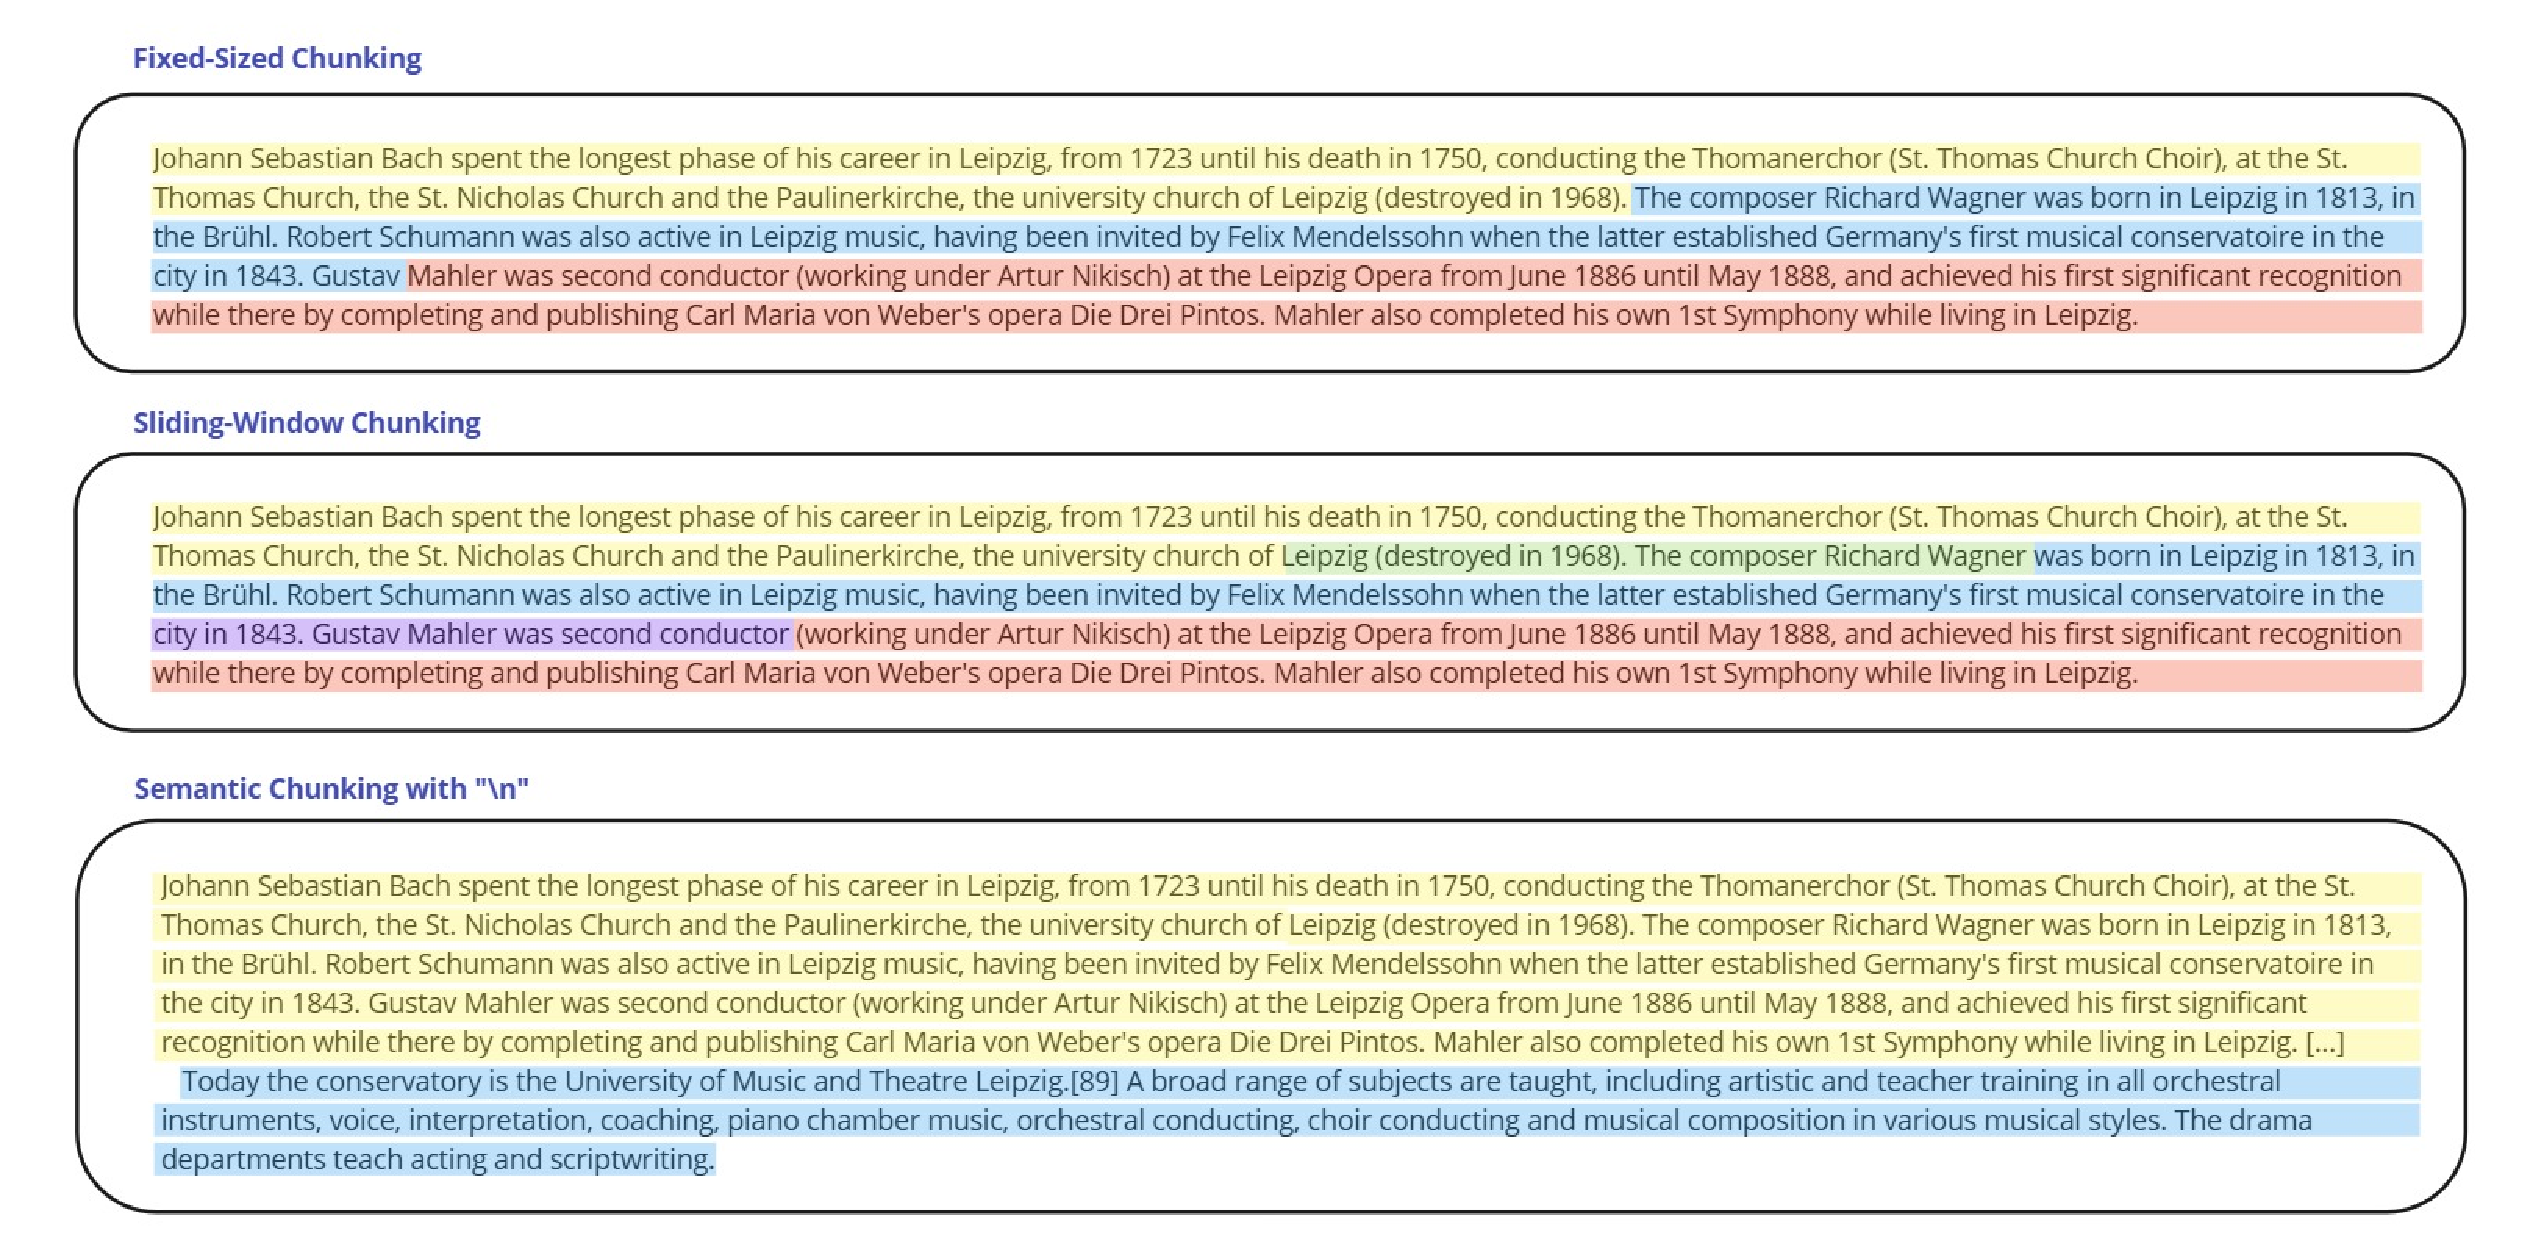
\includegraphics[width=\textwidth]{images/Chunking.pdf}
    \caption{Differnt types of chunking showed on the example of a wikipedia page of Leipzig\cite{LeipzigWikipedia.2025}}
    \label{fig:chunking}
\end{figure}

Therefore there are several chunking techniques to consider for tuning the RAG-system. Fixed-size chunking divides text into uniform segments (e.g., 400-character blocks), while sliding window variants add overlapping regions. The sliding window approach adds a overlap of few characters. Semantic chunking splits with prior defined characters such as "\textit{$\backslash n$, $\backslash\backslash n$ or <br>}". These techniques are visualized in figure \ref{fig:chunking}. There are also special use case techniques such as Markdown, JSON, HTML and programming code chunkers. Almost all presented chunking techniques are offered in typical libraries e. g. Llama-Index \cite{Liu_LlamaIndex_2022} or Langchain \cite{Chase_LangChain_2022}.

% \paragraph{Metadata-Filtering}
% Additional to advanced chunking, it is recommended to enrich the resulting documents with metadata, which can be used at inference time for filtering. 

% ToDo: 
% - Drawbacks
% - Point of Failures in RAGs
% - Überleitung zu Evaluation

\paragraph{Rewrite}
\label{sec:rewrite}
% Query Rewriting, Query Transformation, Query Expansion (see. papers)
\textit{Rewrite} is a collection of pre-retrieval techniques to increase the likelihood of relevant retrieved documents and a concise generation. The query will be transformed, expanded or routed. Query routing in this context describes different RAG pipelines based on the query.\cite{Gao.18.12.2023}

\paragraph{Rerank}
\label{sec:rerank}
% Reranking Techniques, Lost-in-The-Middle?, Diversity Ranking, ... 
\textit{Reranking} mitigates risks which naive RAGs suffer. They key consideration for retrieval is, to decide how many documents should be retrieved. In real worlds scenarios there won't be perfect retrievals. Therefore the retrieval will always introduce noise in form of irrelevant documents or chunks into the generation process. Additional to this, if we retrieve not enough documents, with might risk losing relevant ones that do not appear on the top of the similarity score. Post-retrieval techniques such as rerank mitigate this risk by ranking those documents and order them.\cite{Gao.18.12.2023}


\section{Modular RAG}

There is a variety of different RAG systems with lots of different components. The definition of advanced RAG systems is too strict and sequencial for including this variety. This gap closes modular RAGs. Modular RAGs can be seen as individual component blocks that can be added to a pipeline as long as the input and output of these blocks are compatible. Gao et al. introduced this definition and defined more components then the here presented \textit{rewrite, retrieve, rerank and read}.\cite{Gao.18.12.2023} One simple example of the need of modular RAGs is an routing component, that decides if retrieval is necessary at all. Redirecting to the generator can lead to less computational time and better results in some cases.\cite{Mallen.20.12.2022} This modularity is a key requirements for the ability to build custom RAG systems for each use case.


% \paragraph{IRA Methods}
% \label{sec:IRA}


\subsection{Drawbacks of RAGs}
\label{sec:drawbacks}
Retrieval-augmented Generation systems have several improvements compared to standalone LLMs as describe at the beginning of this chapter. Nevertheless it comes with drawbacks that must be considerd before replacing LLMs in production. 

\begin{enumerate}
    \item RAGs have significantly longer computing times and must be partially computed in sequencial order. Therefore the time-to-first-token (TTFT) is always higher then the vanilla LLM. 
    \item This increase of computing times and the fact that there are more LLM requests for e. g. rewriting or reranking result in higher costs.
    \item RAGs introduce a overhead of work and expertise for developing, maintaining and experimenting with RAGs.
    \item RAGs introduce a high variety of diverse failures in all components of the RAG system. Failures can happen while ingestion too.\\[9pt]
\end{enumerate}

This points show that RAGs are no free lunch and it must be considered if RAG is at all needed for every specific use case. Therefore there is a need for fast RAG experimentation that can address all points necessary for this decision.



\chapter{Related Works}\label{chap:relwork}
\section{RAG Evaluation}

\paragraph{Difficulties in RAG/LLM Evaluation}
Yu, Gan et al.\cite{Yu.2024} note the temporal complexity of information and the need for holistic evaluation methodologies in RAG systems. Ru, Qiu et al. Chang, Wang et al.\cite{Chang.06.07.2023} advocate for specialized evaluations over uniform benchmarks and highlight challenges such as dynamic out-of-distribution evaluation and data contamination. Zhao, Zhang et al.\cite{Zhao.29.02.2024} identify key limitations in RAG systems, including knowledge updates and data leakage, proposing research directions to address these issues. Gao, Xiaong, et al.\cite{Gao.18.12.2023} stress the need for refined evaluation methodologies to keep pace with RAG's rapid evolution and expansion into multimodal domains. 

\paragraph{Component-Specific Challenges and Failures in RAG Systems}
Li et al.\cite{Li.13.01.2025} investigate various design choices in RAG systems, highlighting the superior performance of approaches like Contrastive In-Context Learning RAG and Focus Mode RAG. They emphasize the critical importance of retrieved context quality and prompt formulation over simply increasing the knowledge base size. Liu et al.\cite{JintaoLiu.2024} note the difficulty in locating problems within the RAG pipeline, while Barnett et al.\cite{Barnett.2024} identify seven key failure points in RAG systems, stressing the need for effective validation during operation. Huang et al.\cite{Huang.2023} provide a comprehensive taxonomy of hallucinations in LLMs, discussing their causes and mitigation strategies, and highlight the limitations of current retrieval-augmented systems. Zhao et al.\cite{Zhao.29.02.2024} explore retrieval quality issues, suggesting that excessive retrieval can degrade results. Liu et al.\cite{Liu.06.07.2023} demonstrate that LLMs perform best when relevant information is positioned at the beginning or end of the context, underperforming when it is in the middle. Together, these studies underscore the multifaceted challenges at the component level and illustrate that both design choices and operational failures contribute significantly to the overall limitations of RAG systems.


\paragraph{Evaluation Methodologies and Transparency}
Simon et al.\cite{Simon.10112024} propose a blueprint for reusable empirical study designs for evaluating RAG systems. They emphasize the need for open data for reproducibility while ensuring it remains closed to LLM training to prevent data leakage. The authors also stress the importance of standardized methodologies and transparent reporting to ensure validity and replicability. Wagner et al.\cite{Wagner.12.11.2024} underscore the challenges in reproducing LLM results due to unknown hyperparameters and training data, advocating for transparent yet encoded datasets to enhance reproducibility. Pimentel et al.\cite{M.A.Pimentel.2024} highlight the impact of implementation details on model performance and the need for transparent and standardized reporting of metric calculation procedures to foster reproducibility and comparability across studies. They emphasize that LLM performance is highly dependent on the evaluation methodologies and implementation details used. Overall, these works call for a shift towards greater transparency and standardization in evaluation practices, which is essential for robust performance assessments in RAG systems.

\paragraph{End-to-End Evaluation}

Traditionally, RAG evaluation has primarily relied on end-to-end assessment by comparing the generated output with one or more ground truth references \cite{Salemi.2024}. Although this approach is crucial for gauging overall performance, it suffers from significant limitations when evaluating retrieval models. In particular, end-to-end evaluation lacks transparency regarding which retrieved document contributed to the final output, thereby hindering the interpretability of the system's behavior. 

While end-to-end evaluation provides a holistic view of RAG system performance, understanding the contributions of individual components to the overall system behavior is equally critical. In their comprehensive study, Li et al. \cite{Li.13.01.2025} systematically investigate the intricate relationships between various RAG components and configurations, addressing nine key research questions to unravel the operational mechanisms of RAG systems

\paragraph{Component Evaluation}
The evaluation of generation tasks, especially those involving creativity or open-ended responses, is inherently challenging due to the subjective nature of defining "correct" or "high-quality" outputs \cite{Yu.2024}. To address this, researchers have proposed advanced evaluation methods. For instance, an "Oracle Prompt," which includes all relevant documents, serves as an upper bound for evaluating generation by simulating perfect retrieval conditions \cite{Krishna.19.09.2024}. However, this method can overemphasize retrieval quality by assuming ideal conditions. Li et al. emphasize the widespread adoption of LLMs as judges, noting their ability to align with human judgments while highlighting significant biases, such as preference leakage towards related models \cite{Li.13.01.2025}.

Evaluating the retrieval component of RAG systems presents unique challenges. Ashkan Alinejad et al.\cite{Alinejad.2024} highlight the complexity of assessing retrieval effectiveness by comparing human judgments alongside four evaluation types: Exact Match, Token-Based, Embedding-Based, and LLM-Based. Alireza Salemi and Hamed Zamani\cite{Salemi.2024} introduce eRAG, a novel evaluation framework that leverages downstream task performance to assess retrieval quality more effectively. They demonstrate that traditional relevance labels have a weak correlation with RAG performance, emphasizing the need for task-oriented evaluation methods. Jin et al.\cite{Jin.19.09.2024} reveal that increasing the number of retrieved passages does not consistently improve end-to-end performance, often leading to performance degradation due to hard negatives. To mitigate this, they propose methods like retrieval reordering and fine-tuning techniques to enhance context utilization. Furthermore, Mallen et al. \cite{Mallen.2023} find that retrieving contexts may be unnecessary and even detrimental when dealing with common knowledge, but it benefits questions about rare knowledge, underscoring the importance of contextual relevance in retrieval strategies.

\section{Frameworks and Benchmarks}



\chapter{Designing Generalizable and Reproducible RAG Experiments}\label{chap:design}
% 2. RAG Entwicklung, welche Frameworks gibt es 
% -> Konfigurierbarkeit durch Files
% -> Maintainability
% -> Beliebtheit?
% -> Future Work (Haystack UI)
% -> Modularität (nach Gao.)


Developing retrieval-augmented generation systems is a difficult task that needs several reconfiguration phases.\cite{Simon.10112024} Component evaluation and in-depth failure analysis are key requirements for readjusting the right parts within the RAG-system, as they can include complex pipelines that may involve iterative or recursive processes. Failures can occur in many parts of the RAG-system. Barnett et al.\cite{Barnett.2024} created a list of 7 failures occuring in an advanced RAG system with Rewrite-Retrieve-Rerank-Read (4R) structure as Gao et al.\cite{Gao.18.12.2023} has defined it. Therefore for a framework it is indespensible to evaluate all components next to the end-to-end evaluation for the overall result. In this chapter, we will discuss how RAGs are evaluated accurately in two different aspects - end-to-end evaluation and component evaluation. After that we will discuss how fast RAG development with transparent and reproducible results can be done. We will introduce Haystacks approach of fast modular RAG development. Lastly we will introduce the novelle blueprint by Simon et al.\cite{Simon.10112024} for handling external validity in RAG experiments. 

\section{Evaluation Techniques}

Evaluating retrieval-augmented generation systems is a hard task that is still highly researched. It comes with all machine learning based evaluation problems such as data shifts, generalization errors or data contamination, but has also a variety of failure points introduced by the design of such a complex system. In this section I will introduce a majority of failure points for RAGs and present, how this framework helps to identify them. The final goal of tuning a RAG system is always to maximize its performance in end-to-end evaluation. RAG users want that the response of the systems fully answers its question or completes its task correct. Therefore end-to-end evaluation is important for comparing baselines and thus to decide if a RAG system can be a improvement to standalone large language models. 


The problem that occurs with end-to-end evaluation is that it is far from obvious which parameters we have to tune or which data we have to provide to accomplish a performance improvement. In figure \ref{fig:failures} there is an example for every component in particular RAG system. In reality there are much more points of failures in such systems. We will explore those in section component evaluation.

\begin{figure}
  \centering
  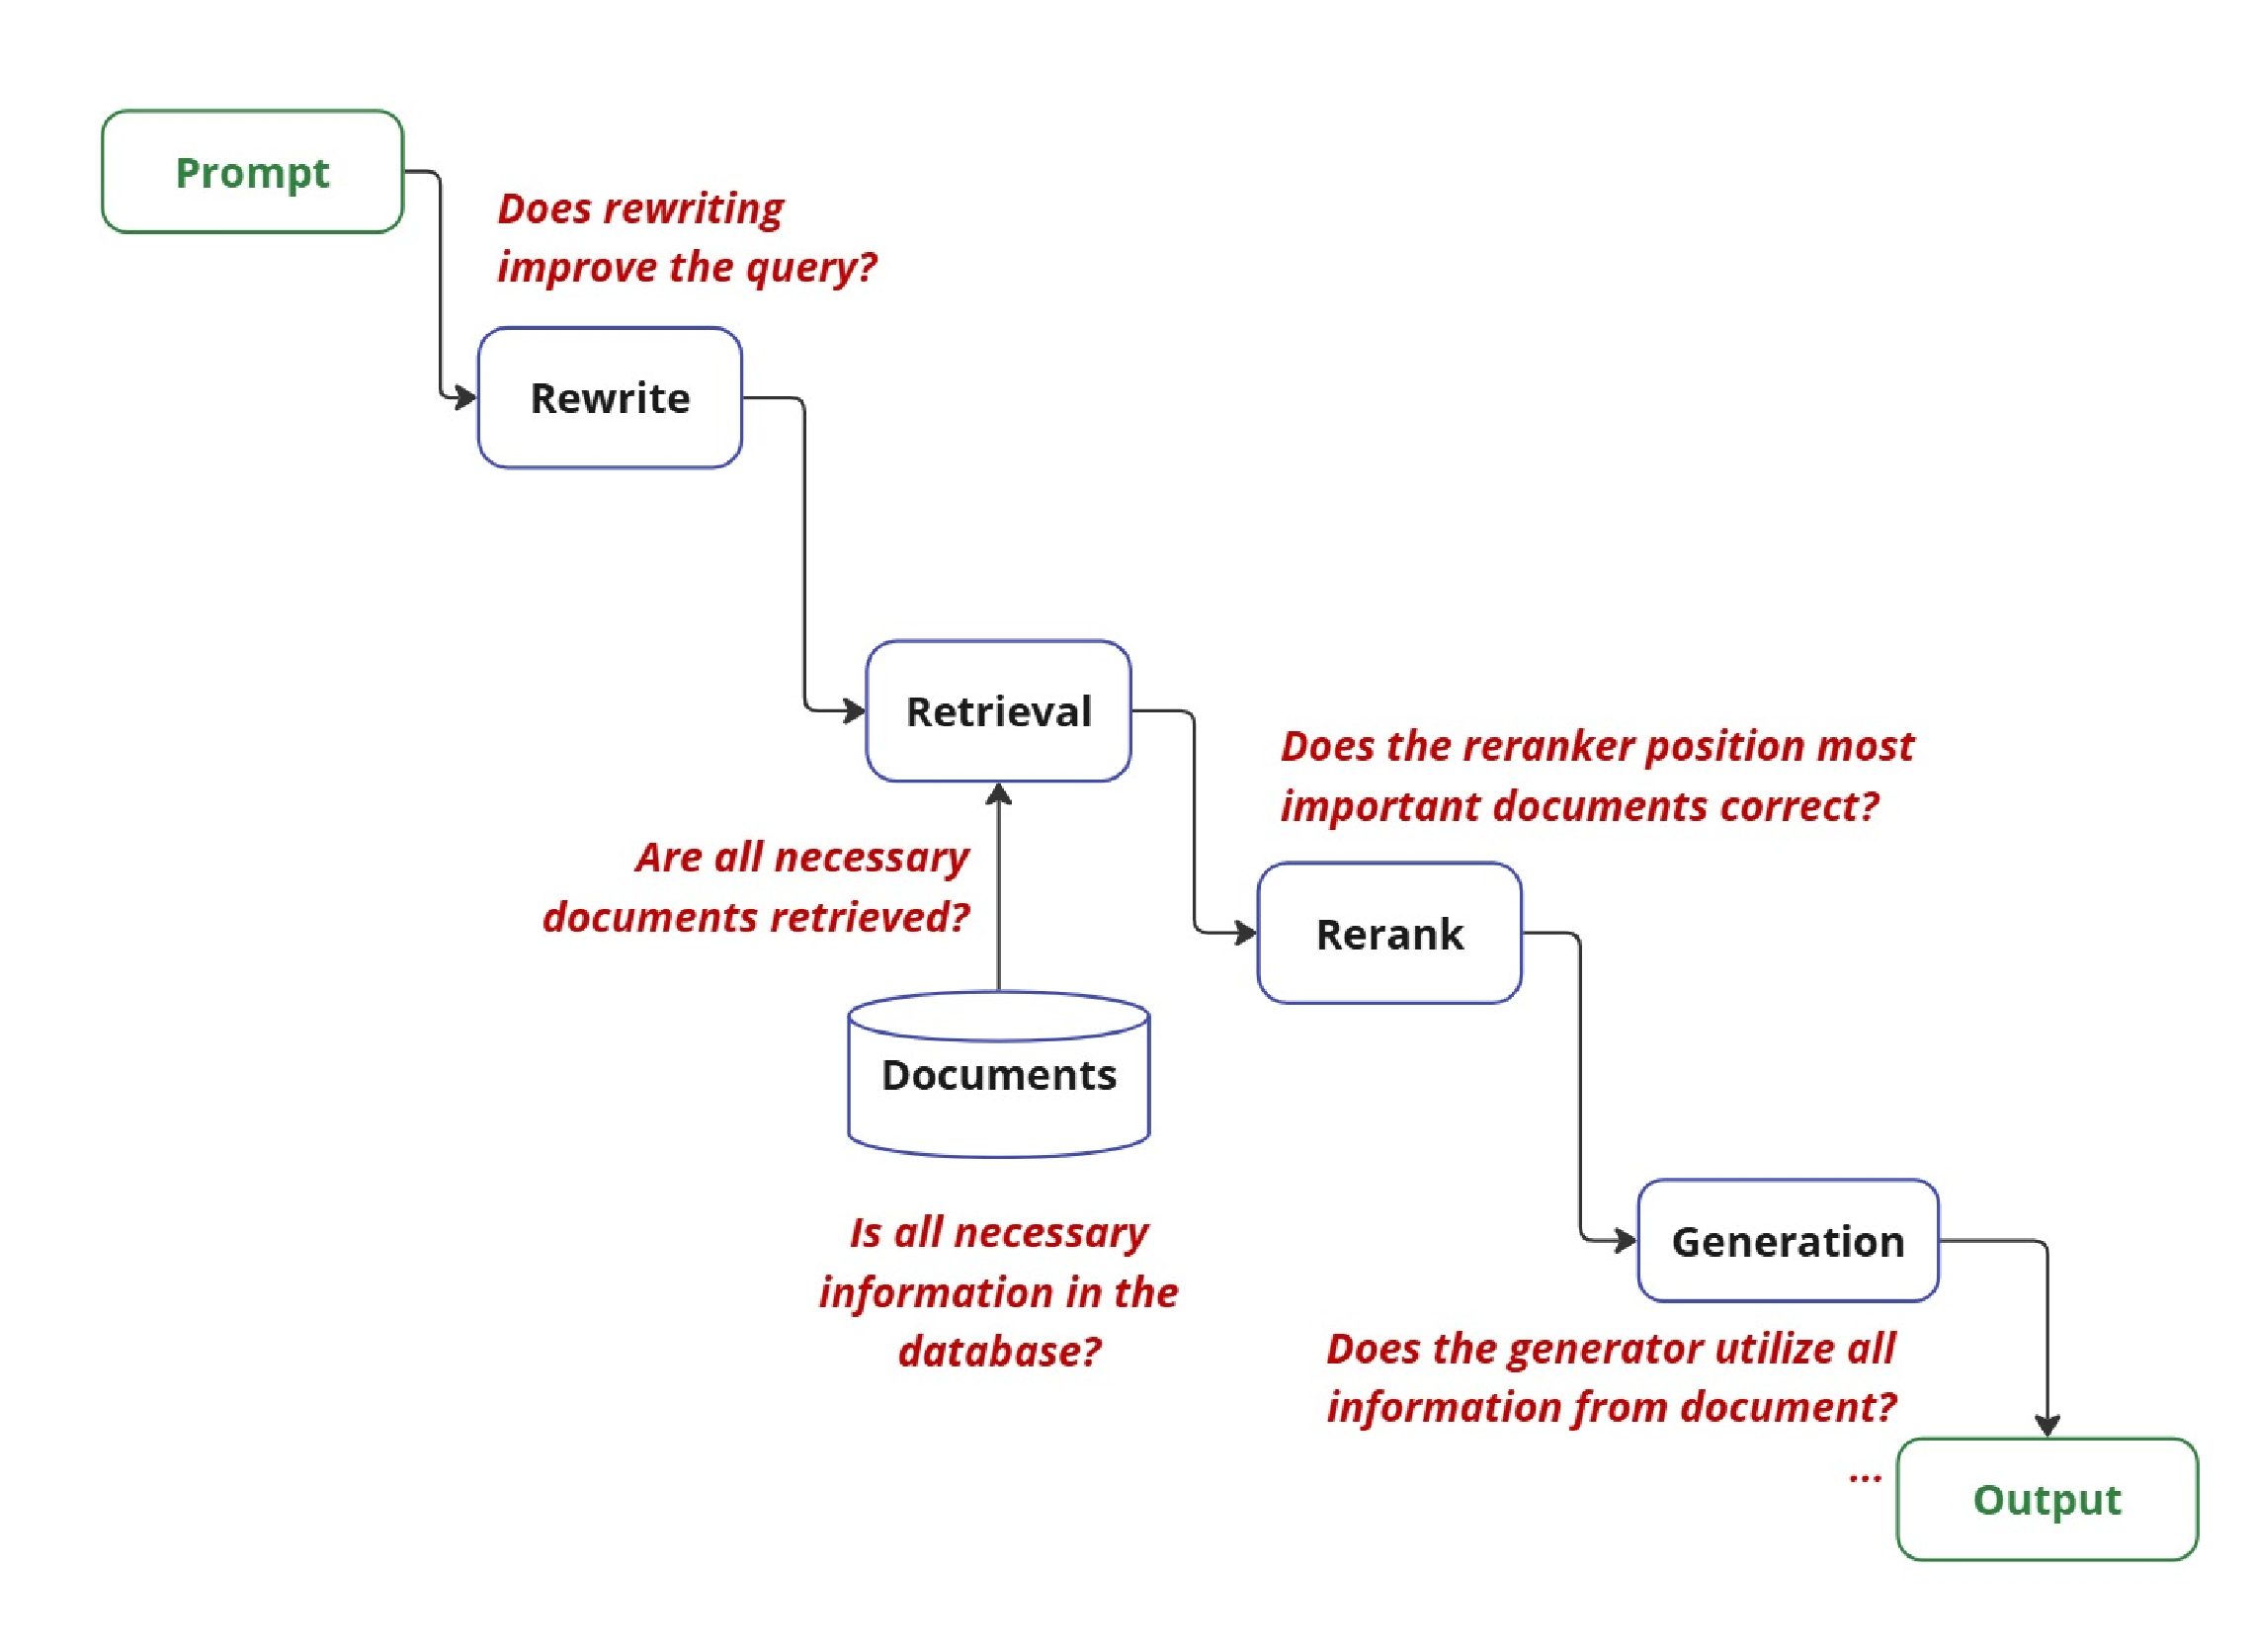
\includegraphics[width=\textwidth]{images/FailurePointExamples.pdf}
  \caption{A RAG pipeline with one failure example of all used components.}
  \label{fig:failures}
\end{figure}

\subsection{End-to-End Evaluation}

We define end-to-end evaluation as metrics that use input and actual output to compare against a ground-truth output to decide if the evaluated item was correct or not. Evaluation that address retrieval are therefore not part of it. In this thesis we will focus on classification tasks only. Therefore the metrics we use for end-to-end evaluations are also limited by classification ones. 

{\renewcommand{\arraystretch}{1.5}%
\begin{table}
  \centering
 \begin{tabular}{|l|l|}
  \hline
  \textbf{Metric} & \textbf{Formula / Description} \\[3pt]
  \hline Accuracy & $\frac{TP + TN}{TP + TN + FP + FN}$\\[5pt]
  \hline Precision & $\frac{TP}{TP + FP}$\\[5pt]
  \hline Recall & $\frac{TP}{TP + FN}$\\[2pt]
  \hline F1-Score & $2 \times \frac{Precision \times Recall}{Precision + Recall}$\\[2pt]
  \hline Matthews Correlation & $\frac{TP \times TN - FP \times FN}{\sqrt{(TP + FP)(TP + FN)(TN + FP)(TN + FN)}}$\\Coefficient & \\[2pt]
  \hline False-Positive Rate & $\frac{FP}{FP + TN}$\\[2pt]
  \hline False-Negative Rate & $\frac{FN}{FN + TP}$\\[2pt]
  \hline Receiver Operating & Curve plotting TPR against FPR at various \\&threshold settings\\[2pt]
  \hline Area under ROC Curve &  AUC of the ROC curve\\[2pt]
  \hline pass@k & Probability of a correct solution in \textit{k} attempts \\[2pt]
  \hline
 \end{tabular}
 \caption{Typical classification metrics used for experiments including RAGs or LLMs\cite{Hou.8212023,Zeng.28.03.2024}}
 \label{table:classification_metrics}
\end{table}}

In stark contrast to evaluating generative tasks, classification comes with clear metrics or methods to evaluate outputs. In table \ref{table:classification_metrics} there is a list of highly used classification metrics for RAG and LLM experimentation.\cite{Hou.8212023,Zeng.28.03.2024} 

End-to-end evaluation requires the researcher to establish a baseline for the experiments. Baslines make experiment results interpretable and ensure that there is something to compare with. Therefore we decided to implement two baselines in this framework, which are used per default if an experiment starts. In the first run, we use the selected generator model alone to get a baseline vs standalone LLMs. Next we run a naive RAG with the data from the predefined corpus, the basic retrieval and generator (retrieve-read, cf: section \ref{sec:naive_rags}). The standalone LLM baseline ensure that the complexity overhead of implementing a RAG system is justified. If the evaluated RAG system can not surpass the performance of the LLM baseline, then simpler system should be used. Similar to that is the naive RAG baseline used to compare more complex RAG variations with more overhead, computation time or costs to the simpler naive one to ensure that the mentioned downsides are justified. 

\begin{figure}[h]
  \centering
  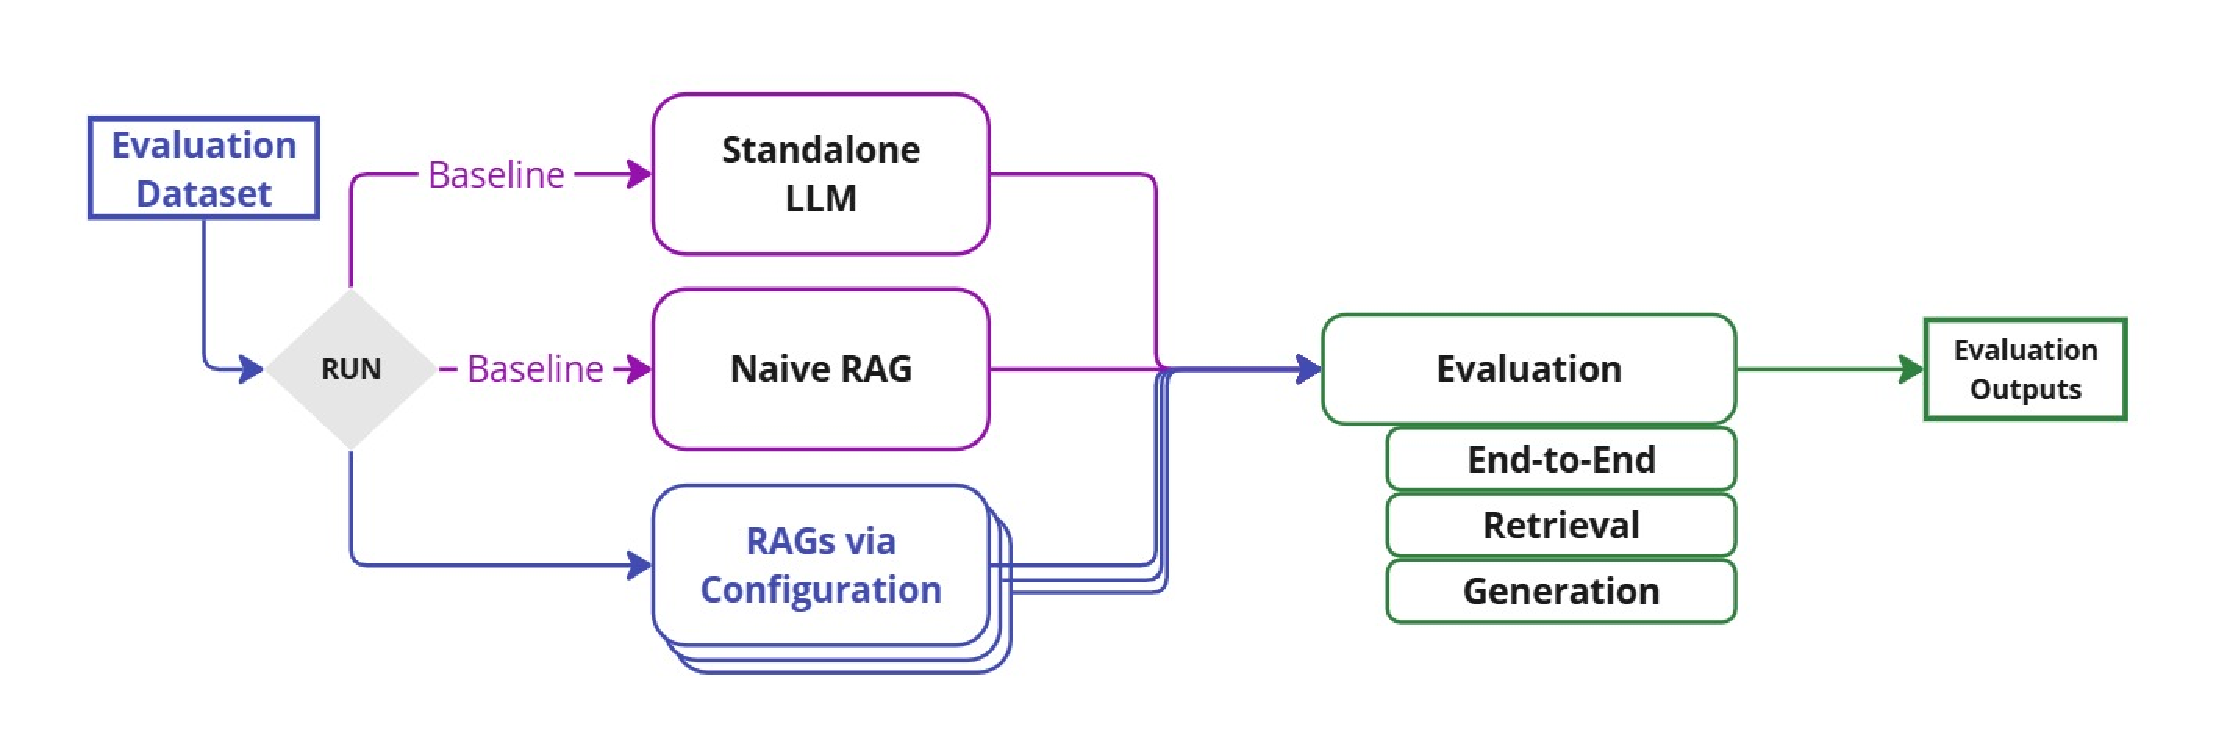
\includegraphics[width=\textwidth]{images/FrameworkBaselines.pdf}
  \caption{Framework: research define configuration files of RAG variations to evaluate them against the baselines standalone LLM and naive RAG with end-to-end evaluation.}
  \label{fig:framework-baselines}
\end{figure}
% \cite{Ru.15.08.2024.} Eventhough all components of a RAG-system affect its overall performance, there are ones that can not be evaluated directly.  \\

We illustrated the prior defined state of our framework in figure \ref{fig:framework-baselines} to enhance the understanding of our considerations. It will be updated with each functionality. It visualizes the process of using our evaluation data to calculate metrics of our baselines next to the configurations we want to test in the experiment. It shows that the evaluation is done by end-to-end as well as component-wise for generation and retrieval. In the following section we will explain, how component evaluation works in our framework.


\subsection{Component Evaluation}

Component evaluation is necessary to detect performance issues of the whole systems introduced through individual components or blocks of components that are connected and do not work well together.\cite{Salemi.2024} In figure \ref{fig:failures}, we presented few of them. While this gives a good first impression of the variety of failures in a RAG system, this visualisation is far from complete. We argue that all components, no matter how small their impact seem, can introduce significant failure rate for the overall system. Therefore it would be necessary to evaluate them all component-wise. 

We are not aware of papers that analyze component evaluation beside retrieval and read - the core components of a RAG system. We also want to make clear, that evaluating components fully isolated by other components is not practical. If we take for example the generator component and want to evaluate it completely apart from retrieval, then we must provide a ground-truth dataset of retrieval chunks. This is doable for easy scenarios in retrieval that need one document chunk e. g. a sentence where a query is exactly answered, but in real-world scenarios there are much more complex cases such as ambigious queries, complex queries or queries that won't need retrieval at all.\cite{Huang.2023} If the researcher adjusts chunk size or technique, then he must also create a new set of ground-truths as the generated documents have changed and the previous selected ones do not exist anymore (cf. section \ref{sec:advanced_rags}). 

If we consider other components then retriever such as rewrite or rerank then there is no ground truth of data. The purpose of rewriting the query is increasing the following retrieval. Therefore the metric is dependend on the retrieval technique too can not be fixed ground truth examples in an evaluation dataset.

The purpose of component evaluation is to find weak spots within the RAG. It is therefore more feasible to evaluate a RAG-system only with system inputs and its ground truth final answers and let a non-deterministic LLM-as-a-Judge evaluate for steps within the RAG-system. LLM-as-a-Judge is a evaluation techniques, where a significantly more performant model or solely on evaluating trained model does the evaluation. Instead of real-valued metrics, an LLM decides and asseses the solution of the task. 

Relying only on system input and ground-truth datasets for evaluation saves a lot of time. Resulting failure analysis of the system and its components must nevertheless rely on tracing single pipeline runs down, which we will discuss in a latter section. In the following sections we will present our evaluation of the retrieval block and the generation block.


\paragraph{Retrieve}
Retrieval Evaluation is possibly the most difficult part in the evaluation for several reasons. First, more retrieval do not imply better results and it is not clear nor obvious which set of documents perfectly serves the generator to give the best answer.\cite{Jin.5222024} Second, in a real world scenario indexed corpus, there are redundant and contradicting information.\cite{Yu.2024} Third, some questions or queries require to view the topic in a diverse manner, highlighting several considerations for different perspectives and fourth, the quality of the query does also affect the retrieval quality, because queries can be too complex and ambigious or not even requiring retrieval, which may also lead to LLM hallucinations.\cite{Huang.2023, Mallen.20.12.2022}

Retrieved documents might contain useful information or not and are therefore binary assessable, enabling metrics that handle \textit{True-Positives, True-Negatives, False-Positives} and \textit{False-Negatives}. However, simple metrics such as recall and precision are not suited to measure the small differences in retrieval.\cite{Yu.2024} There is a need for retrieval evaluation techniques that also capture document rank information.

Additionally there are limitations while working with ground-truths in retrieval evaluation. Ground truth context for a given query might be ambiguously. Selecting a ground-truth set of relevant information is a task that even expert humans are not able to solve perfectly and LLM-as-a-Judge models show high correlation with humans.\cite{Chiang.2023} There is also the problem of changing chunking while reconfiguration. Everytime a chunking technique or parameter is changed, the resulting indexed documents are different too. Therefore it would be required to prepare a new evaluation dataset for ground truth retrievals. This is a great bottleneck for fast reconfiguration cycles, but chunking is a very important parameter to tune. Therefore we will focus in this framework solely on LLM-as-a-Judge evaluation for retrieval to enable chunking parameter tuning.

We utilize a metric called \textit{Context Relevance} (sometimes also referred to as \textit{Context Precision} or similar names in different frameworks), which is fundamentally a Mean Average Precision (MAP) metric employing an LLM-as-a-Judge. This metric assesses the relevance of each retrieved document in relation to a given query. A binary approach is often adopted, where the LLM-as-a-Judge determines for each document whether it is relevant or not. Specifically, frameworks like Haystack's `ContextRelevanceEvaluator`\cite{Pietsch_Haystack_the_end-to-end_2019} implement this binary assessment. For each document, the evaluator determines if it contains any statements relevant to the query. If relevant statements are found, the document is considered relevant (score 1), otherwise not relevant (score 0). The final \textit{Context Relevance} score is then calculated as the mean of these binary relevance scores across all queries, effectively representing a form of Mean Average Precision. While some frameworks like RAGAS might calculate retrieval metrics based on the quality of the generated response, the approach used here and in Haystack focuses directly on evaluating the relevance of the retrieved documents themselves using a binary LLM-as-a-Judge assessment.

We stated before that recall can not fully capture a complex task like retrieval. Therefore we implemented also \textit{Mean Average Precision at K documents MAP@K}, a custom \textit{Context Precision} metric to offer a complementary, rank-agnostic perspective by simply measuring the proportion of relevant documents retrieved. This additional metric ensures a more comprehensive evaluation of retrieval performance, capturing aspects beyond ranking quality.\cite{EvidentlyAIInc..25.02.2025} 

$$MAP@K=\frac{1}{|Q|}\sum_{q=1}^{|Q|}AP@K$$
$$AP@K=\frac{1}{N}\sum_{k=1}^{K}Precision(k) \cdot rel(k)$$
\begin{itemize}
  \item $|Q|$ is the total number of queries in the evaluation set.
  \item $q$ represents a specific query from the set of queries.
  \item $AP@K$ is the Average Precision at K for a specific query.
  \item $N$ is the total number of relevant items for a particular query.
  \item $K$ is the number of top documents being evaluated.
  \item $k$ represents a specific position in the ranked list of retrieved documents.
  \item $Precision(k)$ is the precision calculated at position $k$, defined as the number of relevant items among the top $k$ items divided by $k$.
  \item $rel(k)$ equals 1 if the item at position $k$ is relevant and 0 otherwise.
\end{itemize}

This is a modified version of the \textit{MAP@K}.\cite{Lin.13.10.2020} It is usual to set K very high and let it retrieve a lot of documents to ensure the relevant ones are retrieved. This would be in conflict with the prior defined \textit{Context Precision} metric. Therefore we will only calculating \textit{MAP@K} for the real k value. \textit{Context Precision} measures the retrieval quality based on focussing to retrieve only relevant items and \textit{MAP@K} measures the ranking inside the retrieved documents. A low \textit{Context Precision} and a high \textit{MAP@K} indicate that the paramter \textit{Top-K} can be reduced, because the retrieval works well enough that irrelevant documents appear on the bottom of the retrieval. In contrast a low \textit{MAP@K} could suggest, that the retrieval configurations is not well-adjusted enough, because there are too many irrelevant documents on the top of the retrieved list.

\begin{figure}
  \centering
  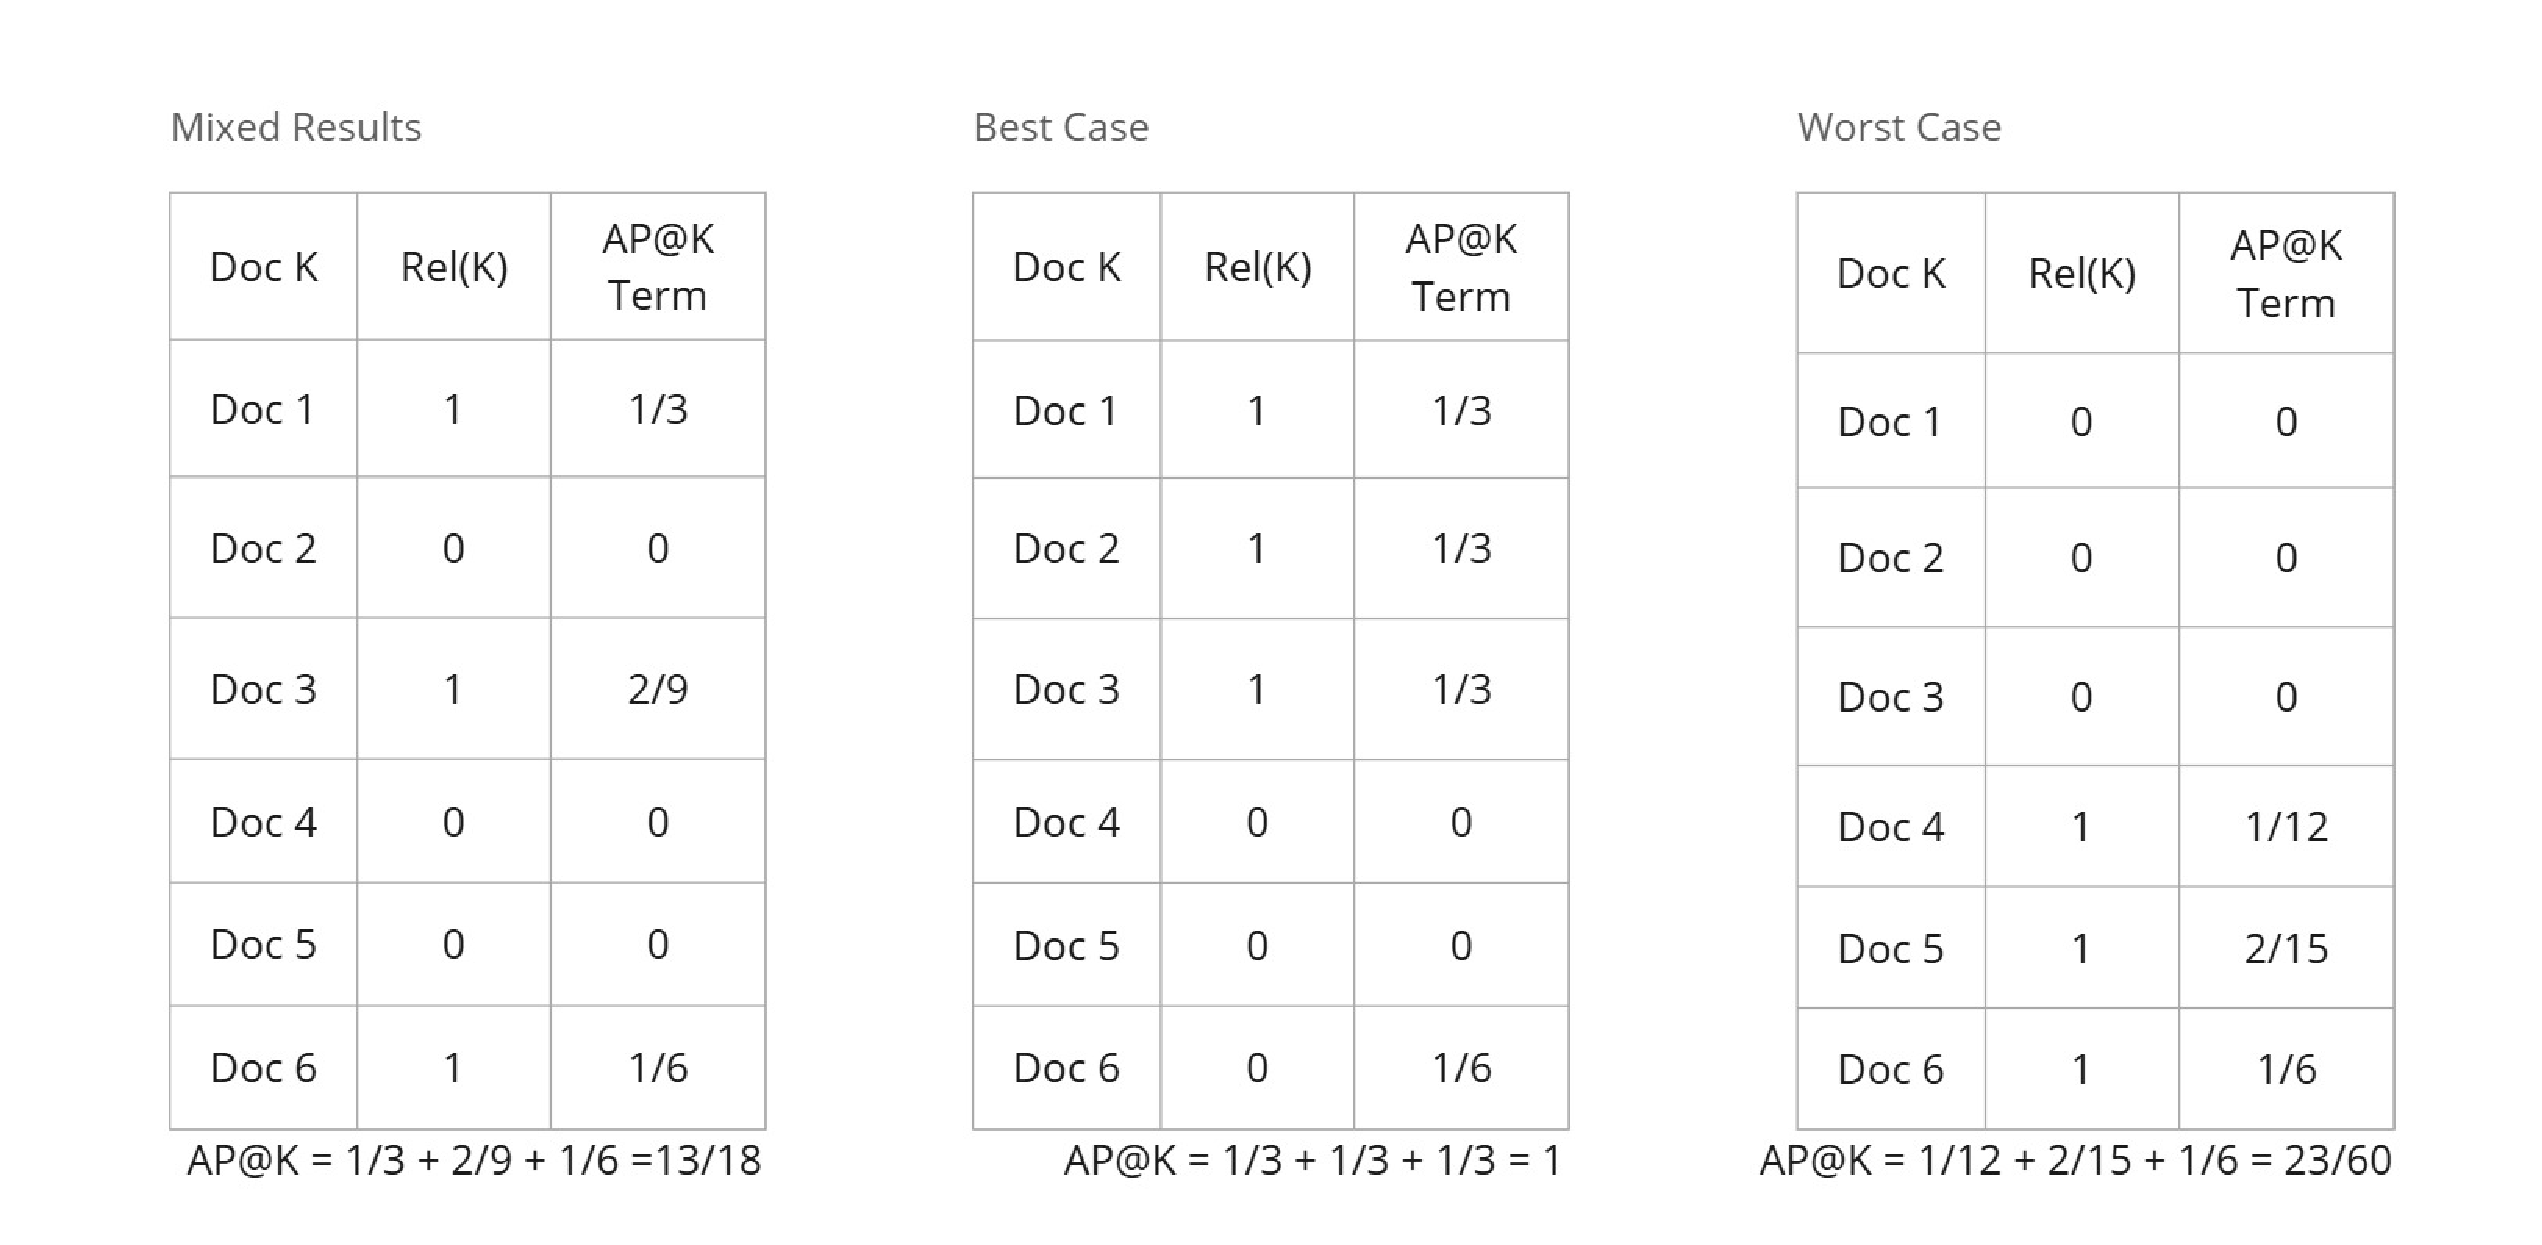
\includegraphics[width=\textwidth]{images/APatK.pdf}
  \caption{This is an example for AP@K metric for one query. At each retrieved document relevance and precision of the first to K-th document will be averaged through all retrieved documents.}
  \label{fig:APatK}
\end{figure}


\paragraph{Generators}
Generators are based on transformer architecture and classification tasks were not the initial intention for this kind of tasks. Thus it is important that outputs are in a wanted form such as \textit{valid}, or \textit{invalid}. Therefore we need a metric that evaluates the generators ability to follow those rules. We call this \textit{format-validator}. The problem that comes with this generator evaluation for classification tasks is that it is impossible to check context utilization, answer relevance based on a simple \textit{True/False} answer. 

Even though the generator only predicts \textit{True/False}, the latent space that lead to this answer have different grades of context utilization and answer relevance. Therefore we will use a slightly different format for the classification task. Instead of generating only binary outputs such as \textit{0} / \textit{1}, \textit{valid} / \textit{invalid} or \textit{True} / \textit{False}, we will also output the reason for it before or afterwards. The only limitation is that the model must generate \textit{'The answer is "True"'}. We implement it with an regular expression.

This has several positive side affects. First, we can measure the reasoning to assess context utilization or answer relevancy, which are important to debug the system. If the context of retrieval is not utilized enough, then we won't figure that out by analyzing binary classes. Second, we enable reasearchers to the current test-time compute paradigm shift for large language models or \textit{large reasoning models}. In practice, they use \textit{<think>...</think>} and use different search algorithms for the best reasoning path before these model answer the query. This leads to significantly better results.\cite{Xu.16.01.2025}


\subsection{Component Block Evaluation}

After evaluating component-wise, we need to evaluate other components, that are not assessable isolated too. In an advanced RAG such a component would be the rewriter. Rewriters try to synergize query to retrieval and context. Defining a performant rewriter depends on whether the RAG uses a sparse or a dense retrieval as he must either use relevant keywords or simulate semantic similarity. The second component from an advanced RAG system would be reranking. Both, reranker and generator have an great impact and interest in context utilization, the ability to build a coherent and correct answer based on actual facts from the retrieved context. Phenomena such as lost-in-the-middle have a significant affect on context utilization, but LLMs differ in this effect.\cite{Liu.06.07.2023} Therefore it might happen that the best reranker and generator regarding their component-wise performance lead to inferior context utilization results. The system needs to be model-agnostic for all components and researchers need rigorous testing of potential component blocks. 

\paragraph{How to evaluate such component blocks?}

\begin{figure}
  \centering
  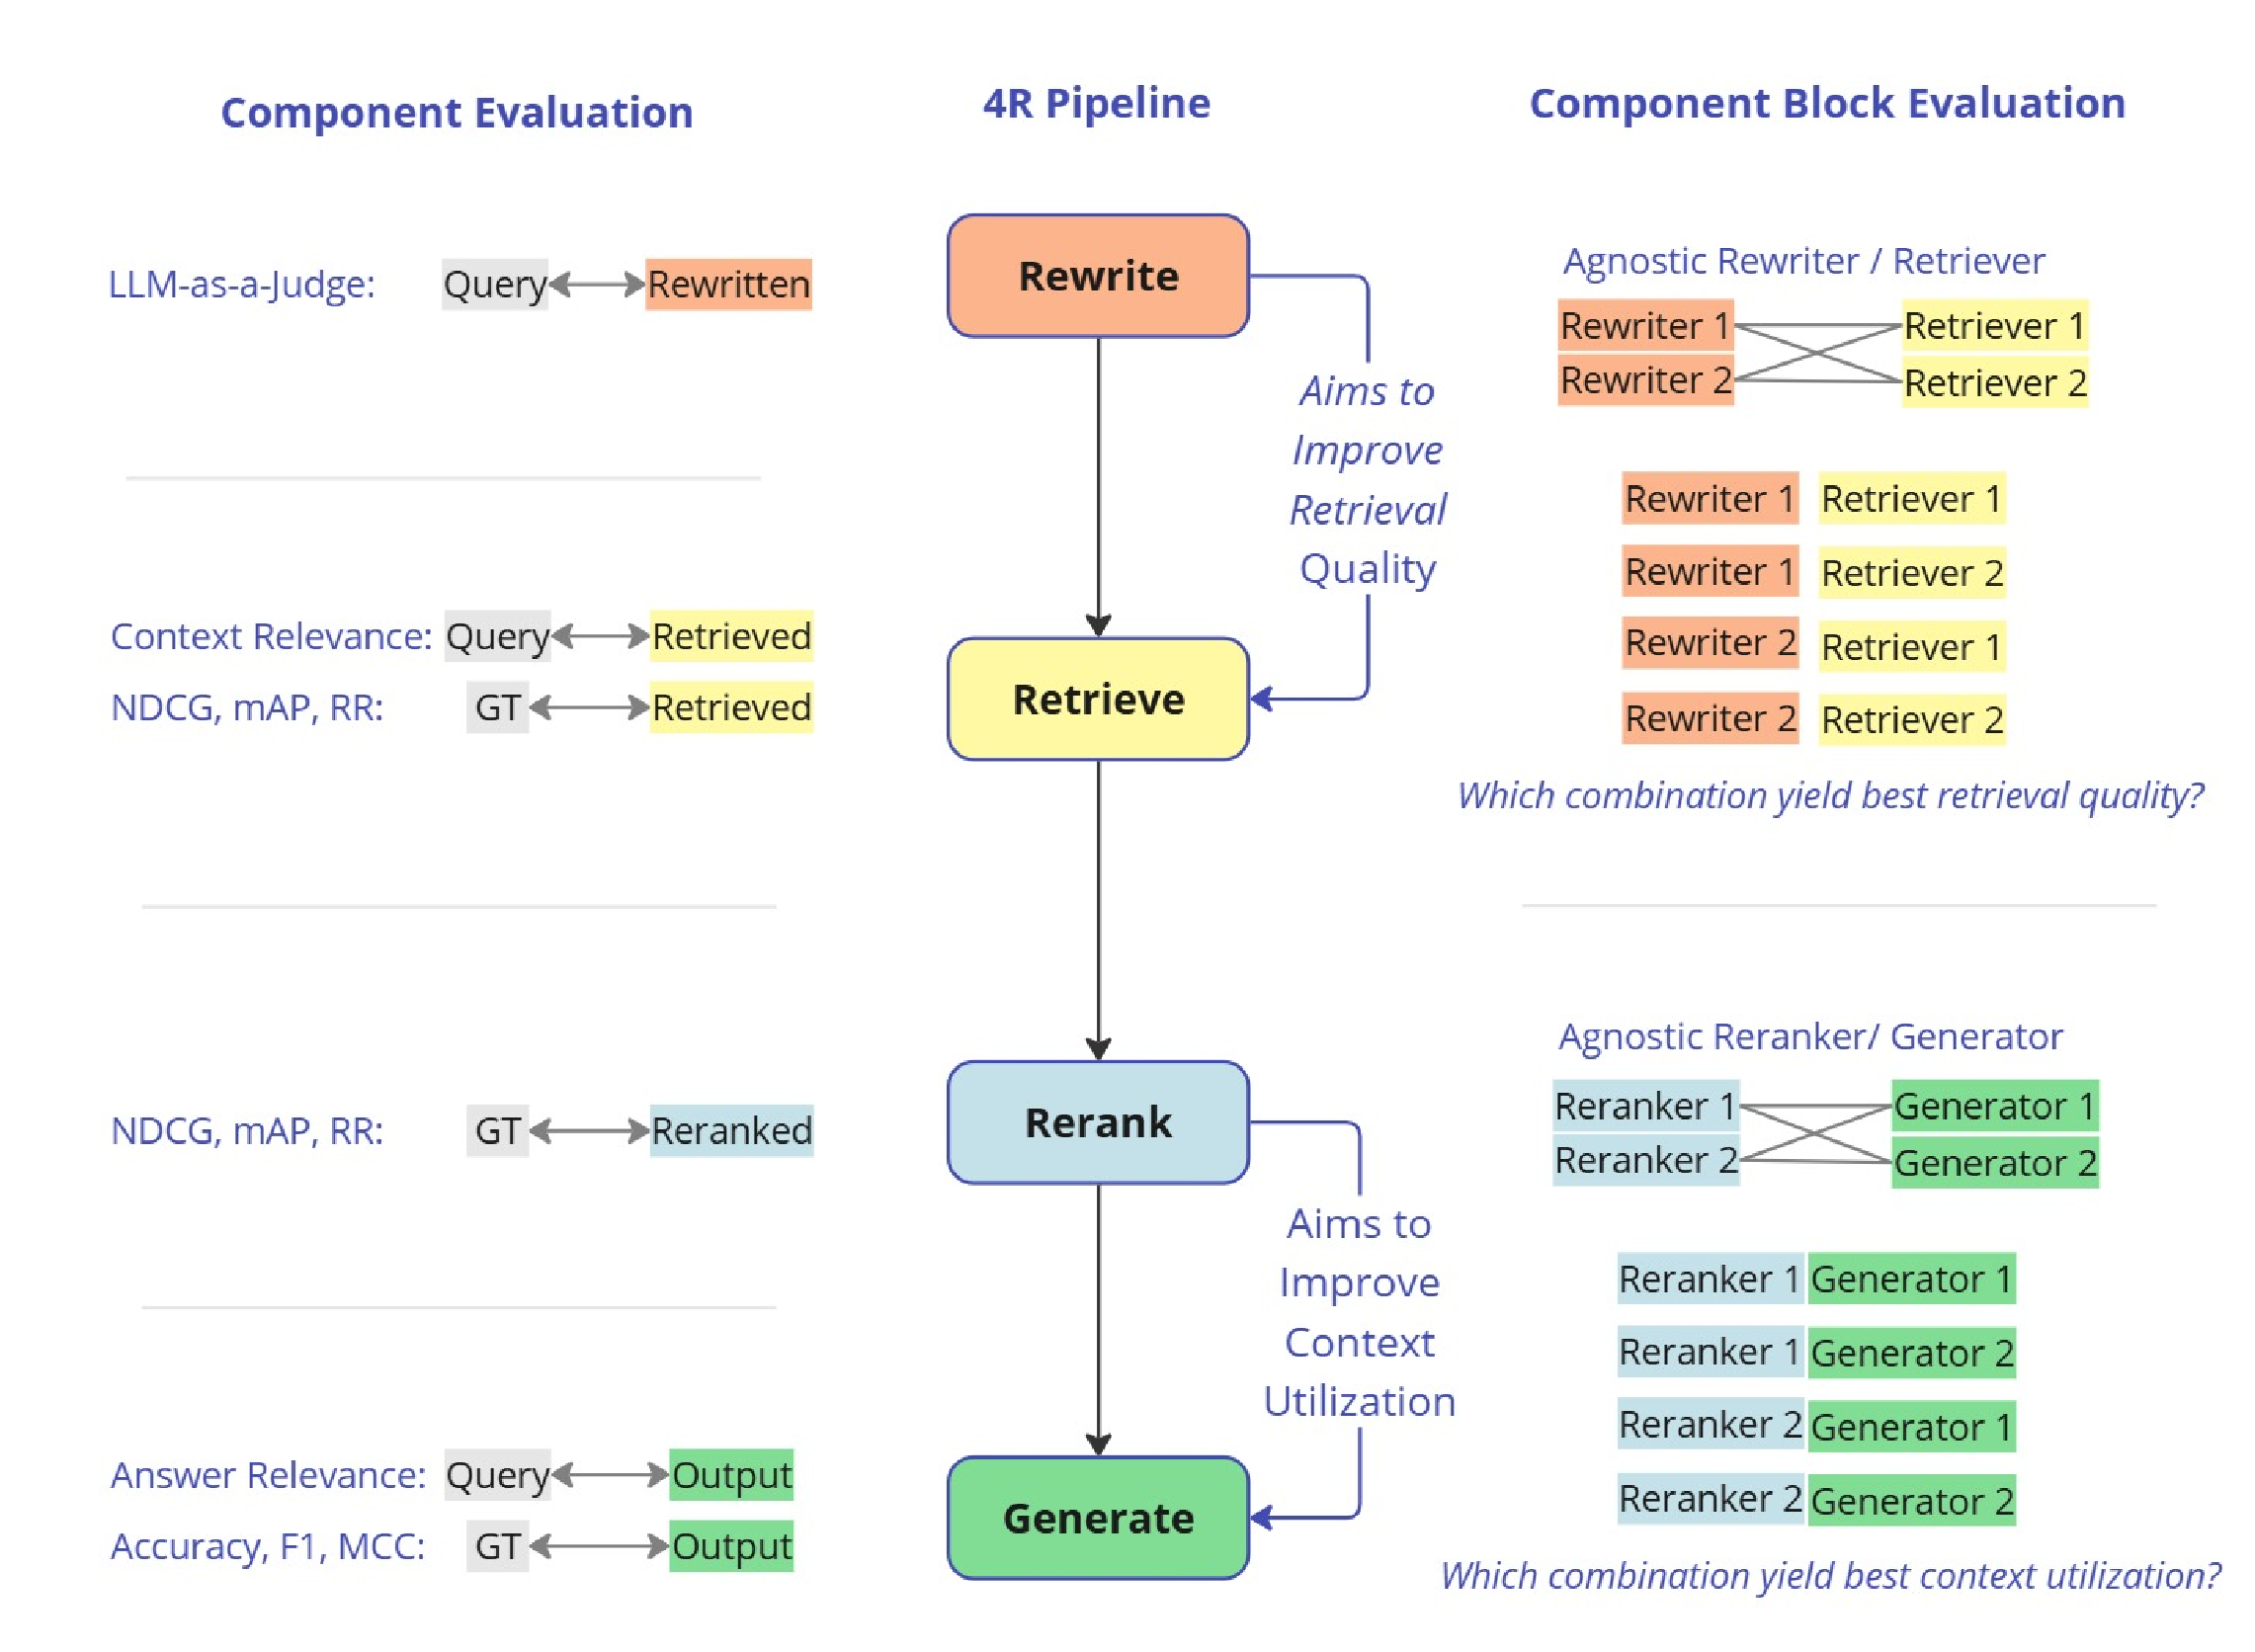
\includegraphics[width=\textwidth]{images/ComponentBlockEvaluation.pdf}
  \caption{Comparison of isolated component evaluation of each component and component block evaluation, where several components with the same goal are evaluated.}
  \label{fig:componentblockeval}
\end{figure}


We differentiate two major blocks - pre-retrieval and post-retrieval. Evaluating pre-retrieval component blocks such as rewriter is a derived task from the retrieval evaluation. The goal of pre-retrieval is to increase the retrieval quality so that the retriever finds all necessary documents or chunks for this task. Commonly used pre-retrieval techniques are query routing, query transformation and query expansion. Even in the ingestion stage, chunking, document selection and preprocessing steps are tuning parameters that influence retrieval results and its quality. 

Post-retrieval components such as reranker aim to improve the context utilization for the generator. The generator requires a curated and limited list of documents that serves its ability and query best. Second, reducing the Top-K parameter for retrievers might result in missing documents with required information. For that we use the same metrics as for the retriever. The additional step of reranking influences the overall performance and evaluating this component is important. 

Most components beside retriever and generator have no direct measurement,there they have to be evaluated by replacement and metrics of the component block. For example, the rewriter is evaluated by using similar components, different models or prompting techniques as rewriter-variations. Then the RAG runs through the evaluation by only changing those rewriter specific configurations. The resulting end-to-end or if applicable the resulting retrieval metrics decide which rewriter setting is better suited.

This requires the researcher to try many different RAG variations for rigorous testing. In the next section we will introduce our appraoch for fast RAG development.


\section{Fast RAG Development}

\begin{figure}[b]
    \centering
    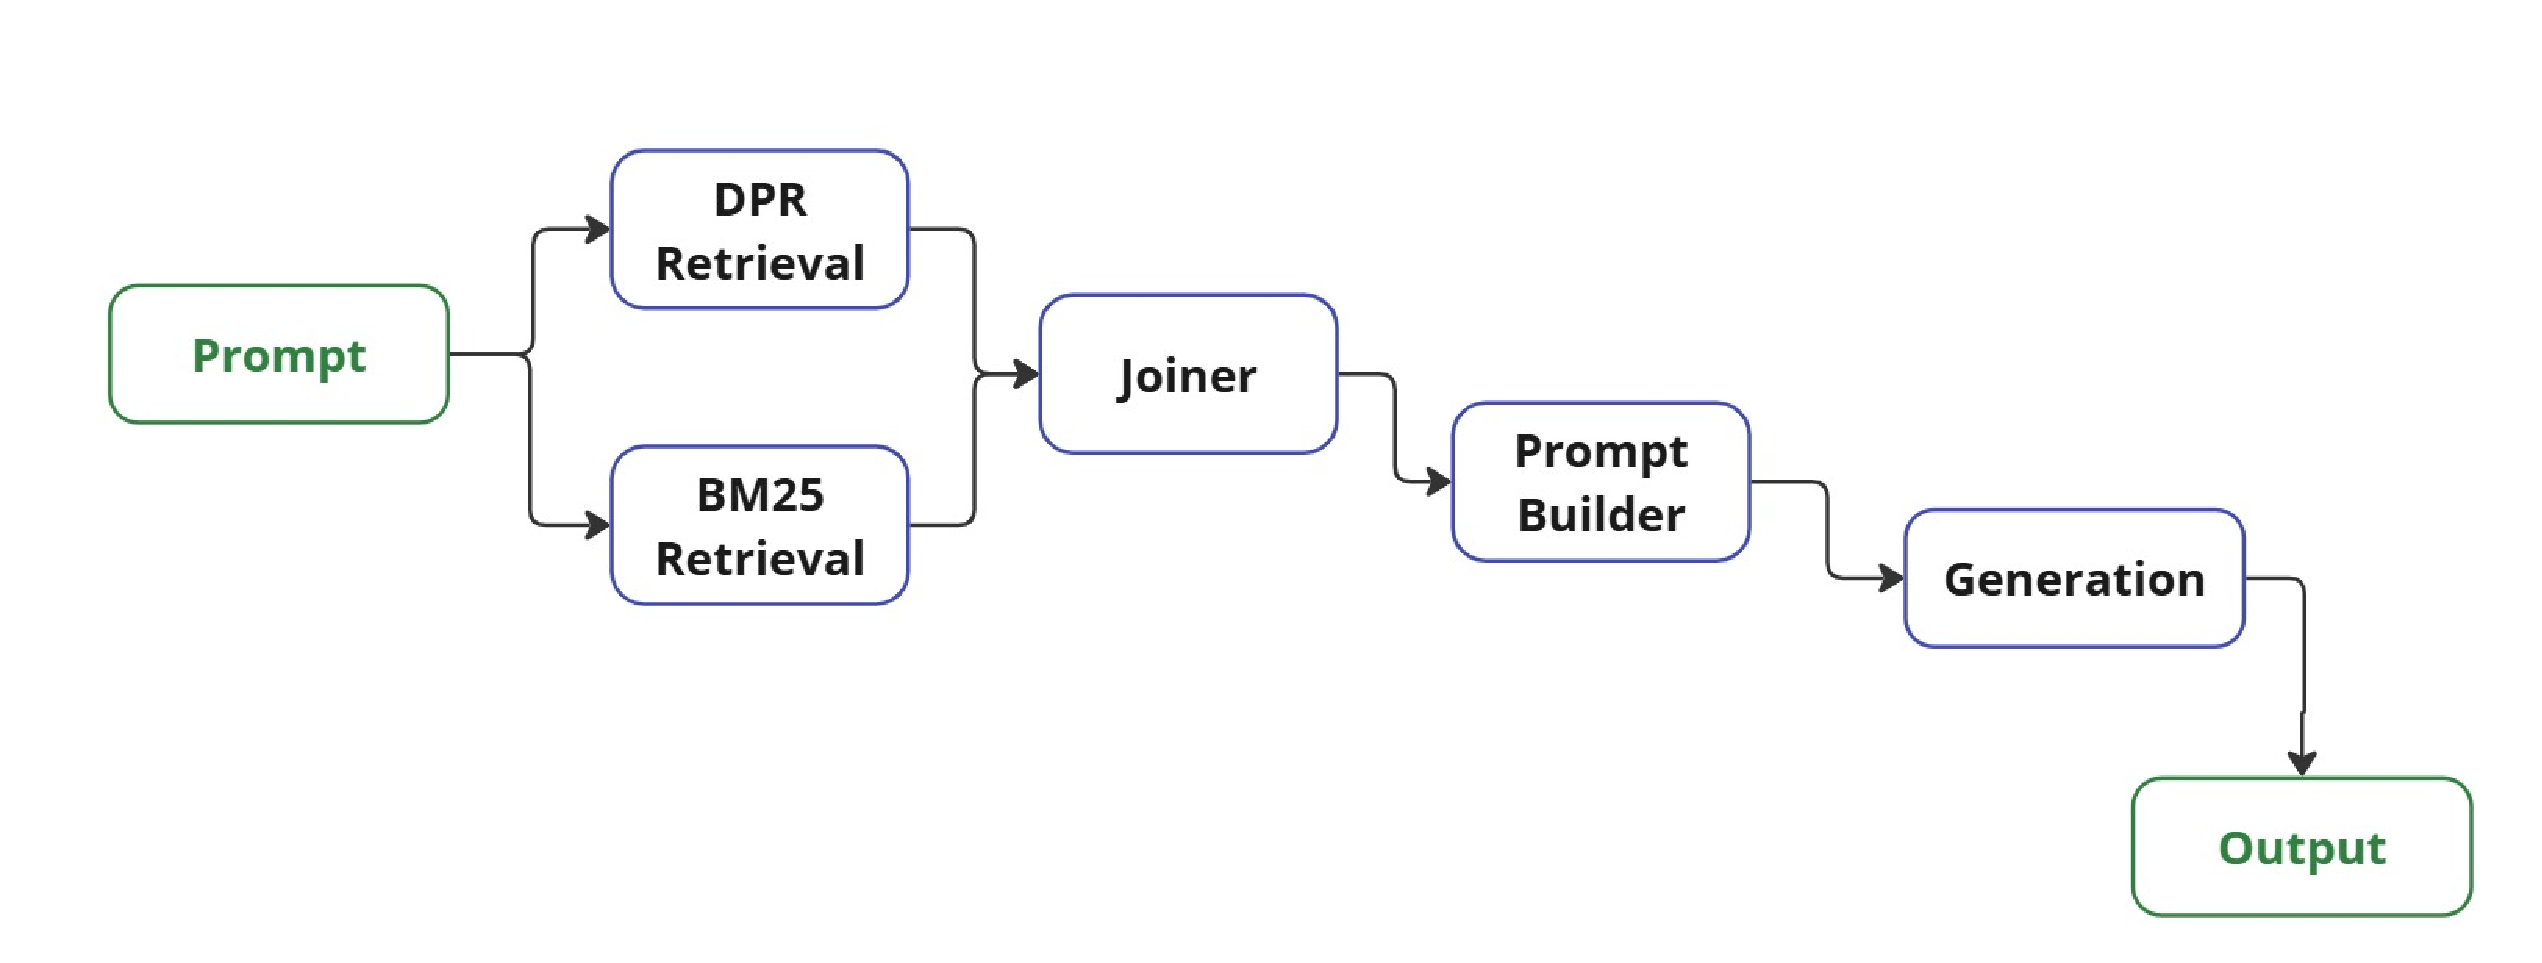
\includegraphics[width=\textwidth]{images/showcase-pipeline.pdf}
    \caption{A simple Retrieve-Read pipeline with both dense and sparse retrieval.}
    \label{fig:showcase}
\end{figure}

RAG systems have a lot of parameters that are not obvious to set. It is common as a researcher to have several reconfiguration phases till the RAG systems works sufficient. More reconfiguration phases lead logically to better results. Therefore Short feedback cycles and fast development make it possible to evaluate many configurations and short feedback cycles can lead to fast bottleneck improvements. This sections presents our considerations for offering fast RAG development.

There are several RAG development tools and frameworks. Highly used ones are Llama-Index\cite{Liu_LlamaIndex_2022}, Langchain\cite{Chase_LangChain_2022} and Haystack\cite{Pietsch_Haystack_the_end-to-end_2019}. All of them offer comparable functionality for building advanced RAG systems in modularized architecture as introduced by Gao et al.\cite{Gao.18.12.2023}. Haystack does offer a functionality, where users can define a pipeline via a YAML-file. This enhances the reconfiguration of such systems, because instead of editing python files, there are just parameters in a YAML to be changed. This enhances the ability to report the methodologies of each experiment too. Instead of saving a python script or module for each configuration, only a YAML is stored that describes the tested RAG architecture fully. An example of this YAML definition can be seen in figure \ref{fig:showcase} and the YAML code below.

Furthermore Haystack comes with router components and the ability to create custom components, which enables iterative, recursive and adaptive RAG functionalities. Components in the Haystack universe can be seen as nodes of an RAG pipeline such as a generator or a retriever. 

\newpage
\begin{minted}[
    frame=single,
    bgcolor=lightgray
  ]{yaml}
components:
  llm:
    init_parameters:
      api_base_url: null
      api_key:
        env_vars: OPENAI_API_KEY
      ...
  prompt_builder: ...
  bm25_retriever: ...
  embedding_retriever: ...
  joiner: ...
  text_embedder: ...
  docs_embedder: ...
connections:
- receiver: llm.prompt
  sender: prompt_builder.prompt
- ...
\end{minted}

\textcolor{red}{Wie werde ich das nutzen? -> Umbauen für Matrix Angabe?}


\section{Reconfiguration}
The visualisation shows the process of reconfiguring the RAG system till its optimized towards a specific validation set. The reconfiguration phase can adjust parameters, using different models, pipelines or even fine-tuning parts such as retriever or generator. We will introduce detailed validity concerns of this common approach in a latter section.


\section{Increasing Transparency in RAG Experiments}

\begin{itemize}
    \item DVC for RAG Experiments
    \item Save YAMLs, Versionize Data + Code
\end{itemize}

\section{External Validity of RAG Experiments}

\begin{figure}
    \centering
    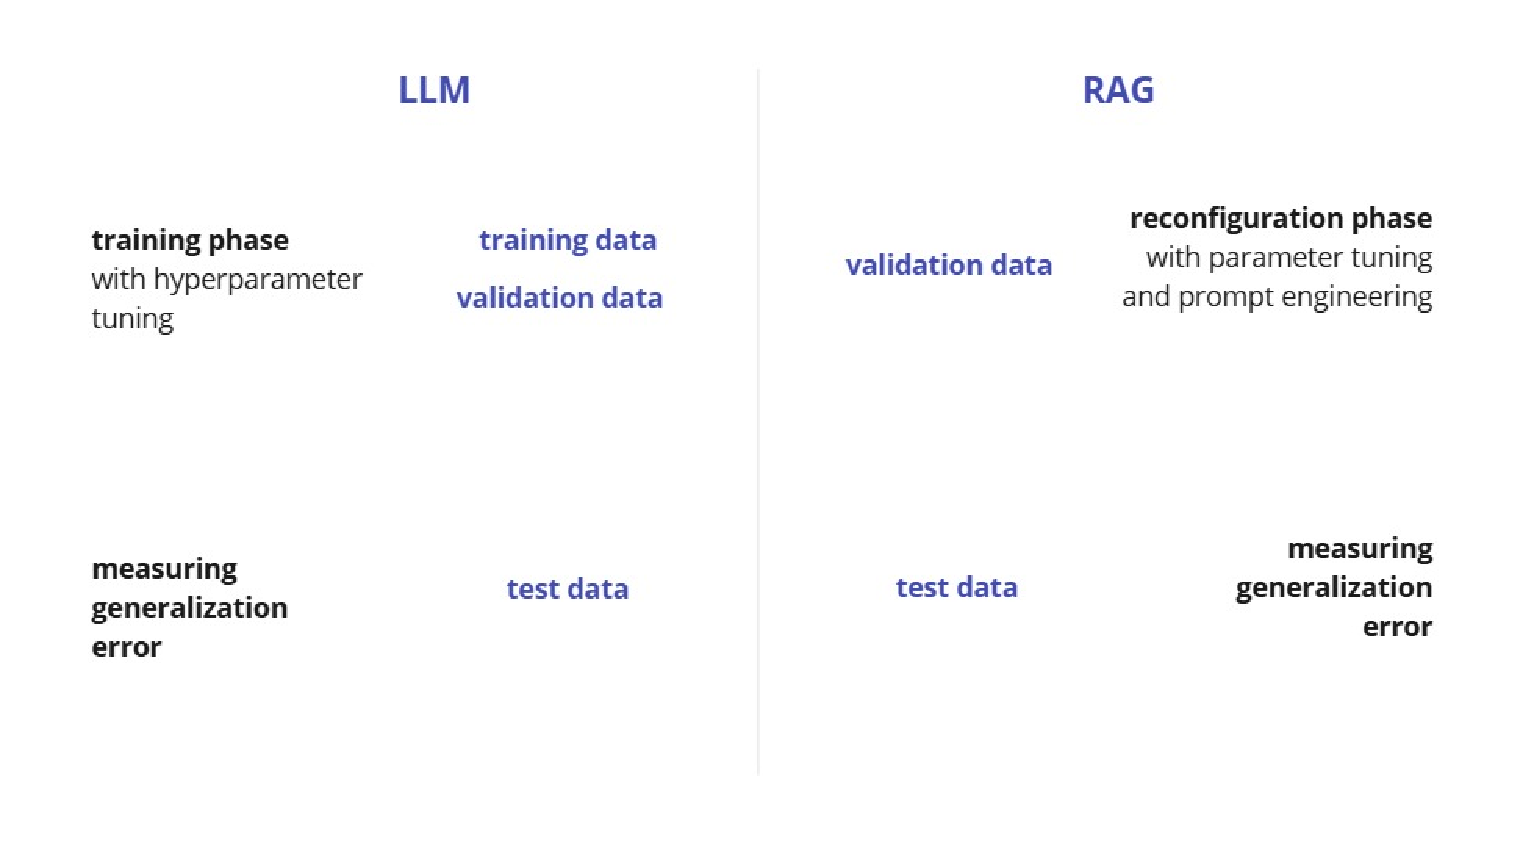
\includegraphics[width=\textwidth]{images/RAGvsLLM-tuning.pdf}
    \caption{Comparison of reconfiguration between RAGs and LLMs - both relying on tuning parameters and test data.}
    \label{fig:tuning}
\end{figure}

% Misconception? RAGs don't need Test-Dataset, because we do not train? But Overfitting is not dependend on training perse, but on free parameter, which happes in RAGs too. Just because we do not have Millions up to Billions of Parameters, does not mean we don't have to consider overfitting. <calculate number of parameters> 


Data is rare, especially for down-stream tasks in domains such as configuration validation or similar tasks. They often rely on few datasets that can not represent the whole domain. Therefore there are measures required to ensure that the developed systems can be generalized from the seen data to the unseen production data. Measuring generalization error in the large language model development is done by splitting the data into training, validation and test datasets. While the training and validation data is used for hyperparameter tuning to ensure the best performing model, the test dataset on the other hand is used to check if the hyperparameter tuning introduced an overfitting. This procedure must be adopted for RAG systems too (cf. figure \ref{fig:tuning}). Even though they do not rely on a training in the most cases, the continous reconfiguration of such systems, including prompt engineering or parameter tuning can lead to differences in seen and unseen data. The needs for a test dataset is independent from a potential training phase, but instead very dependent on a tuning phase for the systems, that is done till the results converge to the best outcoming scenario. Both LLM and RAG development share those reconfiguration phases. 

\textcolor{blue}{Selbst wenn tuning RAGs nicht super anfällig für Overfitting sein sollten, gibt es ja fine-tuning für Retrieval, Generators und Co., welche Overfitting einführen können. Diese werden dann mit dem Objective im RAG bestmöglich zu performen trainiert, daher muss auch da der Generalization Error überprüft werden.}

\paragraph{Preference Leakage}
There are findings suggesting that LLM-as-a-judge favor similar LLMs that their based on. Therefore using synthetic data for evaluation is fast, but risks so called preference leakage.\cite{Li.03.02.2025} 

\paragraph{RAG Evaluation needs a Holdout-Testset}
\begin{itemize}
    \item RAG Experiments belongs to ML Experiments 
    \item Requires Seeding
    \item ML Experiments might cause Overfitting
    \item Generalization (External Validity) is testable with a hard data split (train vs validation vs test)
    \item training data split is not needed, but validation and test is required
    \item validation is for hyperparameter tuning important, which configs have the best results
    \item no testset -> no generalization estimatation
    \item \textcolor{red}{Problem zum Nachdenken} Im Training braucht es ein Holdout-Testset damit man das LLM auswählen kann, welches den geringsten Testfehler hat, aber im RAG wird nicht trainiert. Müssen dann alle Konfigurationen dagegen getestet werden?
\end{itemize}


\section{CLI}

\begin{figure}[!ht]
    \centering
    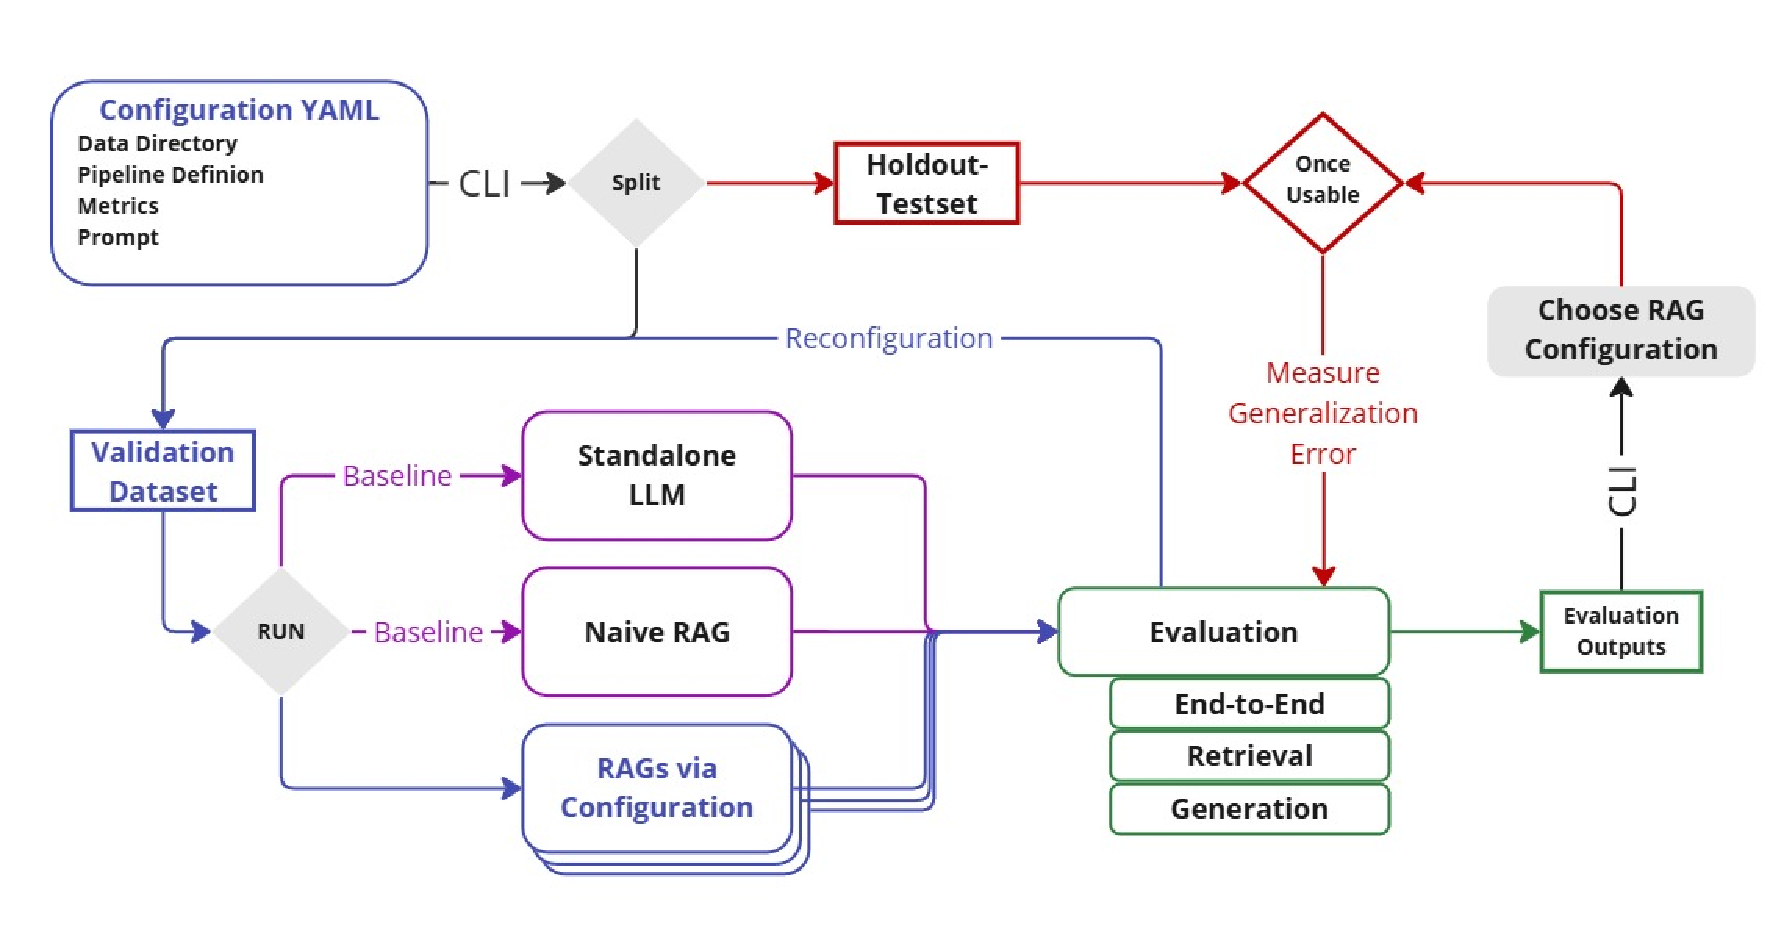
\includegraphics[width=\textwidth]{images/Sketch.pdf}
    \caption{...}
    \label{fig:EvaluationDesign}
\end{figure}

We use the presented Haystack functionalities to build a CLI-based framework around it. Our complete appraoch can be seen in figure \ref{fig:EvaluationDesign}. Given a data directory, pipeline and metrics definition, we first split the data into a validation and holdout-test dataset based on a split parameter \textit{test\_size}. Next we use the resulting validation dataset to run the first evaluations on the data. For that it loads the pipeline and data from its paths and starts with evaluating against a standalone LLM to have a baseline if RAG at all is a significant improvement in contrast to having just an LLM. Next, it ingests data into a vector database and builds an naive RAG with (Retrieve-Read) architecture as another baseline in contast to the in the YAML file defined advanced RAG architecture. The same procedure starts with the RAG configuration from the file. Each run gets evaluated in respect to End-to-End evaluation and component-wise. Evaluations are visualized in \textcolor{red}{EVAL INFOS EINFÜGEN Framework oder PRozess für Indepth Failure Analysis hier erklären}. After failure analysis, the RAG can be reconfigured again to test new parameters. 

\textcolor{blue}{Here comes text how to use Holdout-Test dataset}



\section{Limitations}

List of possible Limitations

\begin{itemize}
    \item Generation Tasks 
    \item Chunking Reconfiguration
\end{itemize}

\chapter{RAG Experimentation on Configuration Validation}\label{chap:Experiment}
\section{Introduction}
Modern software systems involve intricate changes that extend far beyond source code modifications. A significant portion of system behavior is governed by configuration files, encompassing deployment scripts, service settings, infrastructure definitions, and more. Ensuring the correctness of these configurations is critical, yet challenging. Software vendors often provide extensive manuals to guide administrators, but the length and complexity of these documents can be prohibitive, frequently leading practitioners to guess when configuring systems \cite{Xiang.2020}. This challenge is compounded by the rapid pace of technological evolution, which necessitates constant updates to configuration schemes.

The consequences of misconfiguration can be severe, significantly contributing to production bugs and system failures, as highlighted by large-scale studies \cite{Tang.2015}. Traditionally, validating configurations has relied on methods such as static analysis, integration testing, and manual review \cite{Lian.2024}. While valuable, these approaches often struggle to keep pace with the complexity and dynamism of modern software environments. Furthermore, the scale at which validation is required can be immense; Facebook, for example, reported executing trillions of configuration checks daily \cite{Tang.2015}. This necessitates solutions that are not only accurate but also highly performant and resource-efficient, implying that evaluation solely based on metrics like precision or recall is insufficient. Consequently, there is a pressing need for more automated, reliable, and scalable validation techniques.

Retrieval-Augmented Generation (RAG) systems offer a promising approach to address this gap. By combining the knowledge retrieval capabilities of search systems with the reasoning power of Large Language Models (LLMs), RAG can potentially interpret complex technical documentation (like configuration manuals) and apply this understanding to validate specific configurations against best practices or requirements.

This chapter aims to demonstrate the practical application of the RAGBench evaluation framework, detailed in Chapter 4, to the specific problem of configuration validation. We will leverage this framework to systematically evaluate the performance of various RAG configurations against established baselines using an extended version of the CTest dataset \cite{Lian.2024}, which includes synthetically generated examples. While acknowledging that configuration validation is a multifaceted problem involving aspects like inter-configuration dependencies, this experiment focuses specifically on validating individual configuration settings based on documented guidelines.

The remainder of this chapter is structured as follows: Section \ref{sec:related_works_exp} discusses related work in applying RAG to software engineering tasks, particularly configuration validation. Section \ref{sec:exp_design_exec} details the experiment design, including the dataset, baselines, RAG configurations, evaluation metrics, and tools used, adhering to the methodology outlined in Chapter 4. Section \ref{sec:exp_results} presents and analyzes the results obtained on the validation and test sets, including end-to-end performance, component analysis, and failure analysis. Section \ref{sec:exp_discussion} discusses the overall findings and their implications. Finally, Section \ref{sec:exp_conclusion} summarizes the key outcomes of the experiment.
% Note: Added \label tags for section references - adjust as needed if you rename sections.

\section{Related Works} \label{sec:related_works_exp}
Several approaches have been developed for validating software configurations.

Specification-based frameworks, such as ConfValley \cite{Huang.2015}, function by having engineers define validation rules explicitly, often in a declarative manner. Configuration Testing validates configuration values by executing the software components that use these values and observing the resulting program behavior \cite{XudongSun.2020}. This method is used to detect the dynamic effects of configuration settings and identify errors.

Lian et al. \cite{Lian.2024} introduced Ciri, a method that uses Large Language Models for configuration validation. Ciri employs prompt engineering and few-shot learning, providing the LLM with examples of both valid and invalid configurations alongside relevant documentation snippets to identify misconfigurations. This work applies Retrieval-Augmented Generation to the configuration validation task presented by Lian et al. \cite{Lian.2024}. We utilize the RAGBench evaluation framework chapter \ref{chap:design} to systematically assess and reconfigure different RAG systems for this specific task, aiming to optimize their performance through iterative refinement.

\section{Experiment Design and Execution} \label{sec:exp_design_exec}
The following sections detail the design and execution of our configuration validation experiment, adhering strictly to the methodology established by the RAGBench framework presented in Chapter \ref{chap:design}. The core principle involves splitting the evaluation dataset into validation and test sets, performing all system configuration, evaluation, and iterative refinement exclusively on the validation set, and finally assessing generalization on the held-out test set. Specifically, we employ a 70/30 validation-test split for the extended CTest dataset to ensure a sufficiently large test set for estimating generalization error (Section \ref{sec:valtestsplit}).

Our experimental workflow begins by establishing performance baselines using a standalone LLM and a naive RAG system (Section \ref{sec:framework-baselines}). We then evaluate an initial RAG configuration. Subsequent steps involve analyzing performance bottlenecks and failures using the framework's end-to-end and component-level metrics, alongside detailed trace analysis facilitated by MLflow and Langfuse (Section \ref{sec:evaluation-techniques}). Insights from this analysis guide iterative reconfiguration cycles aimed at improving performance on the validation set.

A key difference in our evaluation approach compared to the original Ciri experiment \cite{Lian.2024} lies in handling output formatting. While Ciri reran queries until a correctly formatted answer was obtained, our framework employs a strict format check; if the generator's output does not conform to the expected format (e.g., providing a clear "valid" or "invalid" classification alongside reasoning, as per Section \ref{sec:generator-evaluation}), the response is marked as incorrect for the purpose of end-to-end metric calculation. This reflects a scenario where automated post-processing requires predictable output.

% Differences Ciri to Me:
% They run it as long as it needs to get the correctly formatted answer
% I check with format_checker if the format is correct, otherwise its false

% Start with baselines and an RAG with trivial prompt
% Check for bottlenecks via MLFlow and Langfuse
% <Reiterate here a bit out of the typical experiment workflow showed in 40_DEsign_of_Valid_RAG_Evaluation.tex>

% We will use a 70/30 Validation Test Split for having enough on the test set to estimate correctly


\subsection{Experimental Setup} \label{sec:exp_setup}
The experiments were conducted using the computational resources specified below. The primary environment for running the evaluation framework, including data processing, baseline evaluations, and RAG pipeline executions involving API-based LLMs or CPU-based components, was a dedicated server hosted by Hetzner.

\begin{itemize}
    \item \textbf{Hetzner Server:} [TODO: Insert Hetzner Server Specifications - e.g., Model, CPU, RAM, Disk]
\end{itemize}

For computationally intensive tasks requiring local GPU acceleration, specifically for hosting and running certain large language models, we utilized cloud-based GPU instances provisioned through runpod.io. The vLLM library \cite{Kwon.12.09.2023} was employed for efficient LLM inference on these instances.

\begin{itemize}
    \item \textbf{Runpod.io Instance:} NVIDIA H100 GPU [TODO: Add vRAM amount, e.g., 80GB]
    \item \textbf{vLLM Parameters:} [TODO: Insert key vLLM parameters if non-default, e.g., tensor parallelism, max tokens]
\end{itemize}

The core software components underpinning the experimental setup are provided by the RAGBench framework itself:
\begin{itemize}
    \item \textbf{Haystack:} Used for defining, configuring (via YAML), and executing the RAG pipelines \cite{Pietsch_Haystack_the_end-to-end_2019}.
    \item \textbf{MLflow:} Employed for logging experiment parameters, configurations (including YAML metadata), and evaluation metrics (end-to-end and component-level) for visualization and comparison \cite{MLflow}.
    \item \textbf{Langfuse:} Utilized for capturing detailed execution traces of the RAG pipelines, enabling in-depth failure analysis \cite{Langfuse}.
    \item \textbf{Vector Database:} We use two different vector databases: ChromaDB and In-Memory for estimating the effect on a external database as used in practice.
\end{itemize}


\subsection{Reconfiguration Phases} \label{sec:exp_results} % Renamed section slightly to better reflect content
% Present and discuss the results obtained using ONLY the validation dataset. 


\paragraph{Dataset} % Added subsection for Dataset description
% Describe the dataset used for evaluation.
% Source, size, characteristics.
% Mention the validation-test split ratio (e.g., 80/20) and justification (Sec 4.1). - Already mentioned split ratio earlier.
[TODO: Describe the extended CTest dataset - source, size, format, types of configurations covered, how it was extended (synthetic data?)]

\paragraph{Initial Configuration and Baselines} \label{sec:exp_initial_config}
This section details the performance of the baseline systems and the initial RAG configuration evaluated on the validation set. 

\subparagraph{Baselines}
Two baselines were established as per the framework's methodology:
\begin{itemize}
    \item \textbf{Standalone LLM:} We want to use three different models for baselines: OpenAI's gpt-4o-mini\cite{OpenAI_2022}, Google's gemma-24b \cite{Gemma3.25.03.2025} and Alibaba's QwQ-32B\cite{qwq32b,qwen2.5}
    \item \textbf{Naive RAG:} A simple retrieve-read pipeline using BM25 retrieval over the documentation corpus and the same LLM as the standalone baseline (using \textit{gpt-4o-mini} and a Top-K of 10)
\end{itemize}

\textcolor{red}{Hier kommt auch das CIRI Experiment mit GPT-3.5. Das einzige nutzbare Model für mich, da die anderen zu teuer wären.}

\subparagraph{Initial RAG Configuration} % Describe the specific RAG configuration tested first.
The first RAG system evaluated employed a straightforward configuration:


\paragraph{Reconfiguration I} \label{sec:exp_reconfig_1}
Based on the analysis of the initial configuration, the first reconfiguration phase focused on ...


\paragraph{Reconfiguration II} \label{sec:exp_reconfig_2}


\paragraph{Reconfiguration III} \label{sec:exp_reconfig_3}

\subsection{Generalization Test} \label{sec:exp_generalization}
% Present the results of the final selected configuration(s) on the held-out test set (Sec 4.1, Sec 4.6).
% Compare test set performance against validation set performance for these configurations.
% Use tables/figures.
% Discuss any significant differences and potential signs of overfitting.

\subsection{Discussion} \label{sec:exp_discussion}
% Interpret the overall results of the experiment.
% Which configuration performed best overall?
% Did the RAG systems outperform the baselines?
% Was the added complexity of advanced RAG justified?
% Discuss the implications of the findings for the specific task (configuration validation).
% Acknowledge limitations of the experiment (e.g., dataset size, scope of configurations tested).

\subsection{Conclusion} \label{sec:exp_conclusion}
% Summarize the main findings and contributions of this specific experiment.
% Reiterate the performance of the best RAG system found.


\chapter{Conclusion}\label{chap:Conclusion}
The advent of Large Language Models (LLMs) has revolutionized natural language processing, yet their inherent limitations, such as knowledge cutoffs, potential for hallucination, and difficulty accessing private or rapidly changing information, necessitate more robust solutions for many real-world applications. Retrieval-Augmented Generation (RAG) systems have emerged as a promising approach to mitigate these issues by grounding LLM responses in external knowledge sources. However, as explored throughout this thesis, this approach presents its own significant trade-offs. The integration of retrieval mechanisms introduces significant complexities, increased inference times, and new challenges in evaluation and optimization.

This thesis addressed these challenges by considering two central questions: "Is an advanced RAG system necessary for a given use case, or is a standalone LLM sufficient?" and "How can one determine if a specific RAG configuration is optimal for its intended task?" The primary contribution of this work is the development and demonstration of RAGnRoll, a comprehensive benchmarking framework designed to facilitate systematic and reproducible RAG evaluation.

RAGnRoll, detailed in Chapter \ref{chap:design}, provides a structured methodology to navigate the intricacies of RAG development. Key features of the framework include:
\begin{itemize}
    \item \textbf{Systematic Baselining:} The framework mandates the evaluation of standalone LLMs and naive RAG configurations as baselines (as argued in Section \ref{sec:e2e}). This crucial step helps quantify the added value of more complex RAG architectures and informs the decision of whether RAG is beneficial for the specific task and dataset.
    \item \textbf{Rigorous Validation and Generalization Assessment:} Inspired by standard machine learning practices, RAGnRoll enforces a strict validation-test split of evaluation data (Section \ref{sec:valtestsplit}). All system tuning and iterative reconfiguration are performed exclusively on the validation set, with the test set reserved for a final assessment of generalization error, thereby mitigating the risk of overfitting to the development data, a critical concern when tuning complex RAG systems.
    \item \textbf{Comprehensive Multi-faceted Evaluation:} Recognizing that RAG performance is multi-dimensional, the framework supports both end-to-end evaluation and granular component-level analysis. This allows for the identification of bottlenecks within the RAG pipeline. Furthermore, this thesis argues for and the framework design accommodates the inclusion of hardware metrics (e.g., latency, resource utilization) alongside traditional accuracy-based metrics, providing a holistic view of a system's practicality.
    \item \textbf{Transparent and Reproducible Experimentation:} Leveraging tools like MLflow for results logging and Langfuse for detailed execution tracing (Section \ref{sec:ui}), RAGnRoll promotes transparency and aids in in-depth failure analysis. The use of Haystack's declarative pipeline configurations further enhances reproducibility.
\end{itemize}

The practical utility and effectiveness of the RAGnRoll framework were demonstrated in Chapter \ref{chap:Experiment} through an experiment focused on software configuration validation. This application showcased how the framework can guide the iterative development and comparison of different RAG systems, leading to optimized configurations tailored to specific requirements, including considerations for output formatting and computational overhead.

The practical application in Chapter \ref{chap:Experiment} served to demonstrate RAGnRoll's core functionalities. However, the breadth of RAG configurations explored in that instance was necessarily guided by the project's timeframe and resources. The reported experiments, with an approximate cost of 200 Euro, highlight the framework's utility for initial, cost-effective investigations. A key strength of RAGnRoll is its design for scalability; with more extensive time and financial backing, it can be readily employed to systematically evaluate a far wider spectrum of embedding models, generation models, and intricate RAG architectures than was feasible within the direct experimental scope of this thesis. This underscores its potential for larger-scale research or industrial deployment.

In conclusion, this thesis provides both a conceptual blueprint and a practical implementation for the robust evaluation of RAG systems. By emphasizing systematic comparison, rigorous testing for generalization, comprehensive metric collection, and detailed failure analysis, the RAGnRoll framework empowers researchers and practitioners to make data-driven decisions in the rapidly evolving landscape of retrieval-augmented generation. It offers a path to move beyond ad-hoc tuning towards a more principled approach to building effective and efficient RAG solutions, ultimately helping to answer whether a RAG system is indeed necessary and how to best configure it for a specific use case.

\section{Roter Faden ...}
RAG seems to be a free lunch (see paper with RAG vs Long Context LLMs), but isn't. 
\begin{itemize}
  \item System more complexity increased
  \item Inference Time increased
  \item Only useful in some scenarios 
  \item Hard to evaluate because of its many parts
  \item ...
\end{itemize}

All items are interesting in this thesis. The background ellaborated on the variety of advanced RAG techniques and here the conclusion would be that an evaluation framework should include hardware metrics next to performance metrics for measuring the overhead of the RAG compared to a standalone LLM. The usefulness is measured by the three stage evaluation through LLM, Naive RAG, Advanced configured RAG. Here it would be important to point out the failure points within a RAG system, as it was showed in lecture of Prof. Siegmund too. 
% Appendix
\appendix
% \section*{Custom Component}

% \begin{minted}[
%     frame=single,
%     breakanywhere,
%     breaklines
% ]{python}
% from haystack import component, Document
% from typing import List
% import asyncio

% @component
% class DocumentSummarizer:
%     """
%     A component generating summaries for each given document
%     """
%     prompt = """You are a helpful assistant, that summarizes documents very concisely.\n\nSummarize the following document:\n{document}\n\nSummary:"""

%     async def summarize(self, doc: Document):
%         # Summarizing Code

%     @component.output_types(documents=List[Document])
%     def run(self, documents: List[Document]):
%         """Run the component in parallel for multiple documents"""
%         async def async_run():
%             tasks = [self.summarize(doc) for doc in documents]
%             results = await asyncio.gather(*tasks)
%             return {"documents": results}
%         return asyncio.run(async_run())


% \end{minted}


% \newpage

\chapter{Pipeline Diagrams}

\begin{figure}[h]
  \centering
  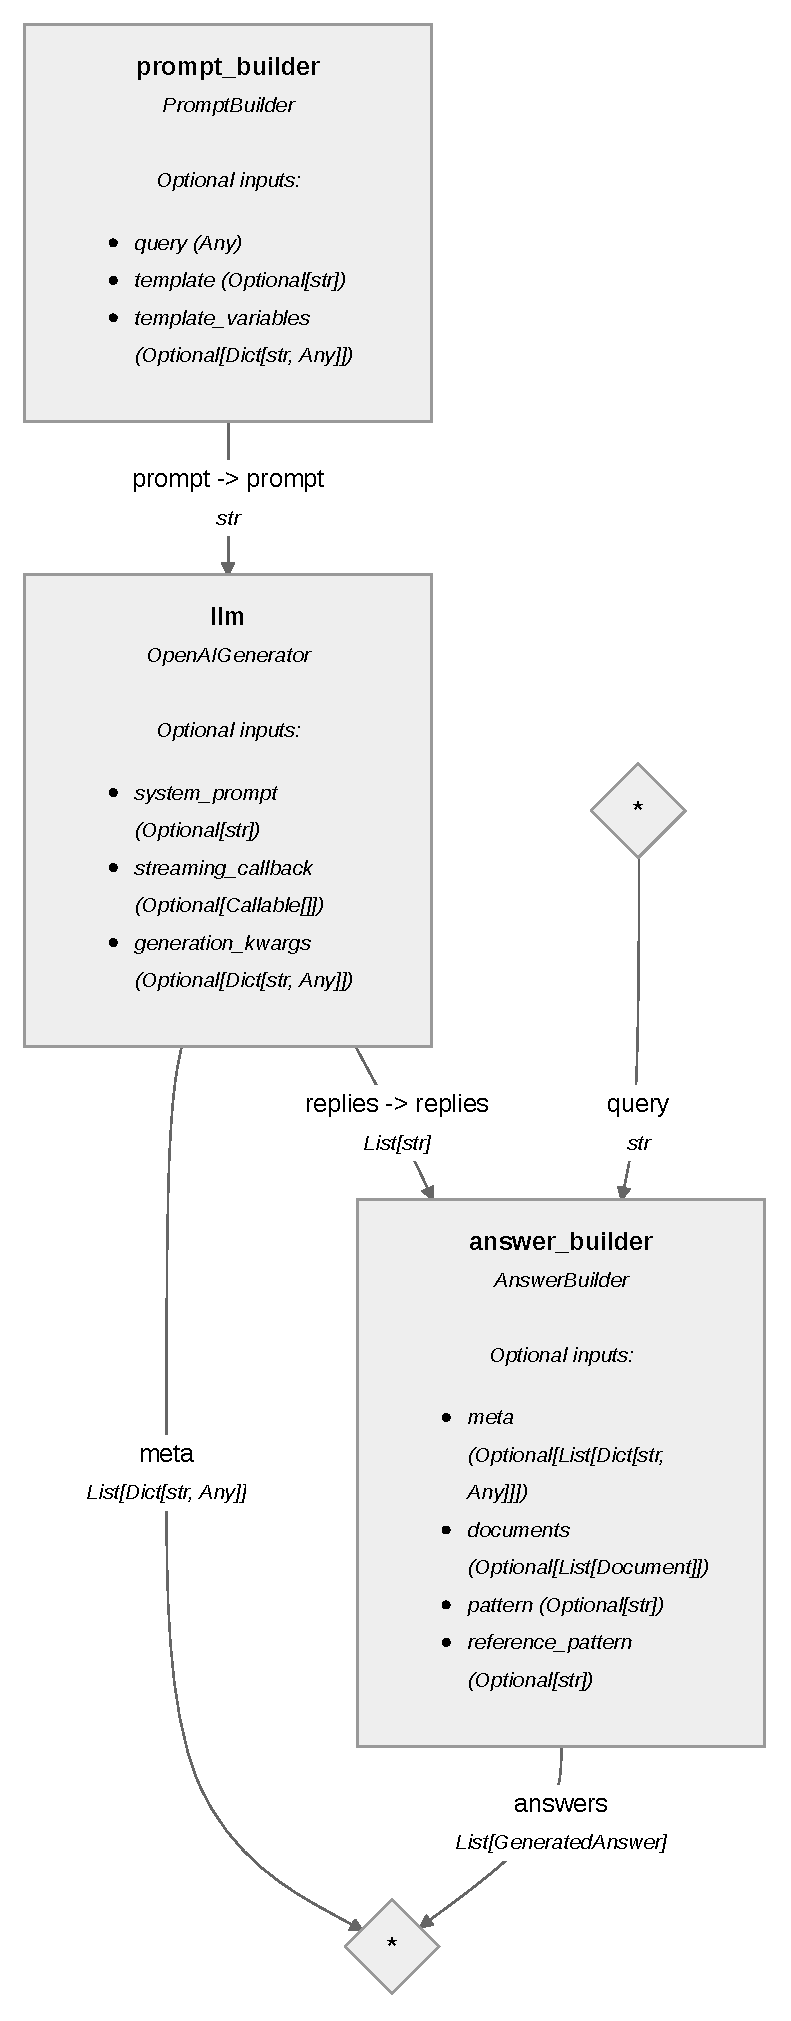
\includegraphics[width=0.35\textwidth]{images/baseline_llm.pdf}
  \caption{Pipeline diagram of the standalone LLM baseline implementation}
  \label{fig:pipeline_llm}
\end{figure}

\newpage

\begin{figure}[h]
    \centering
    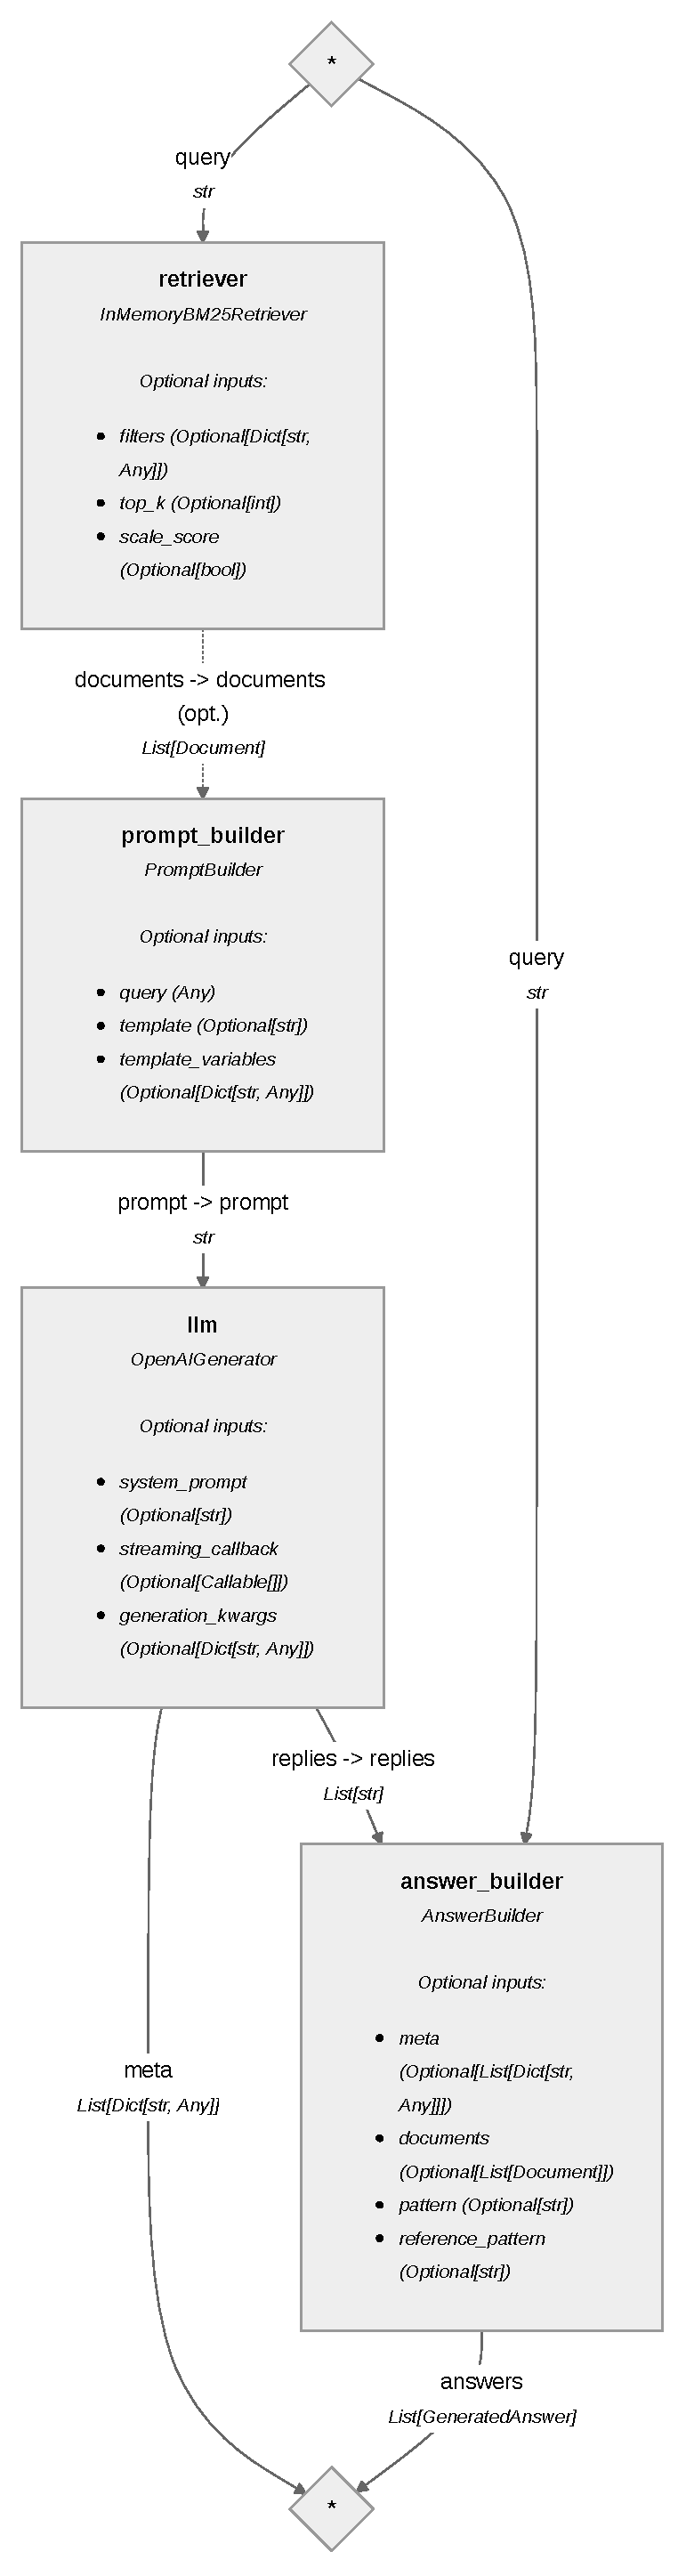
\includegraphics[width=0.37\textwidth]{images/baseline_bm25.pdf}
    \caption{Pipeline diagram of the BM25 baseline implementation}
    \label{fig:pipeline_bm25}
\end{figure}


\newpage

\begin{figure}[h]
    \centering
    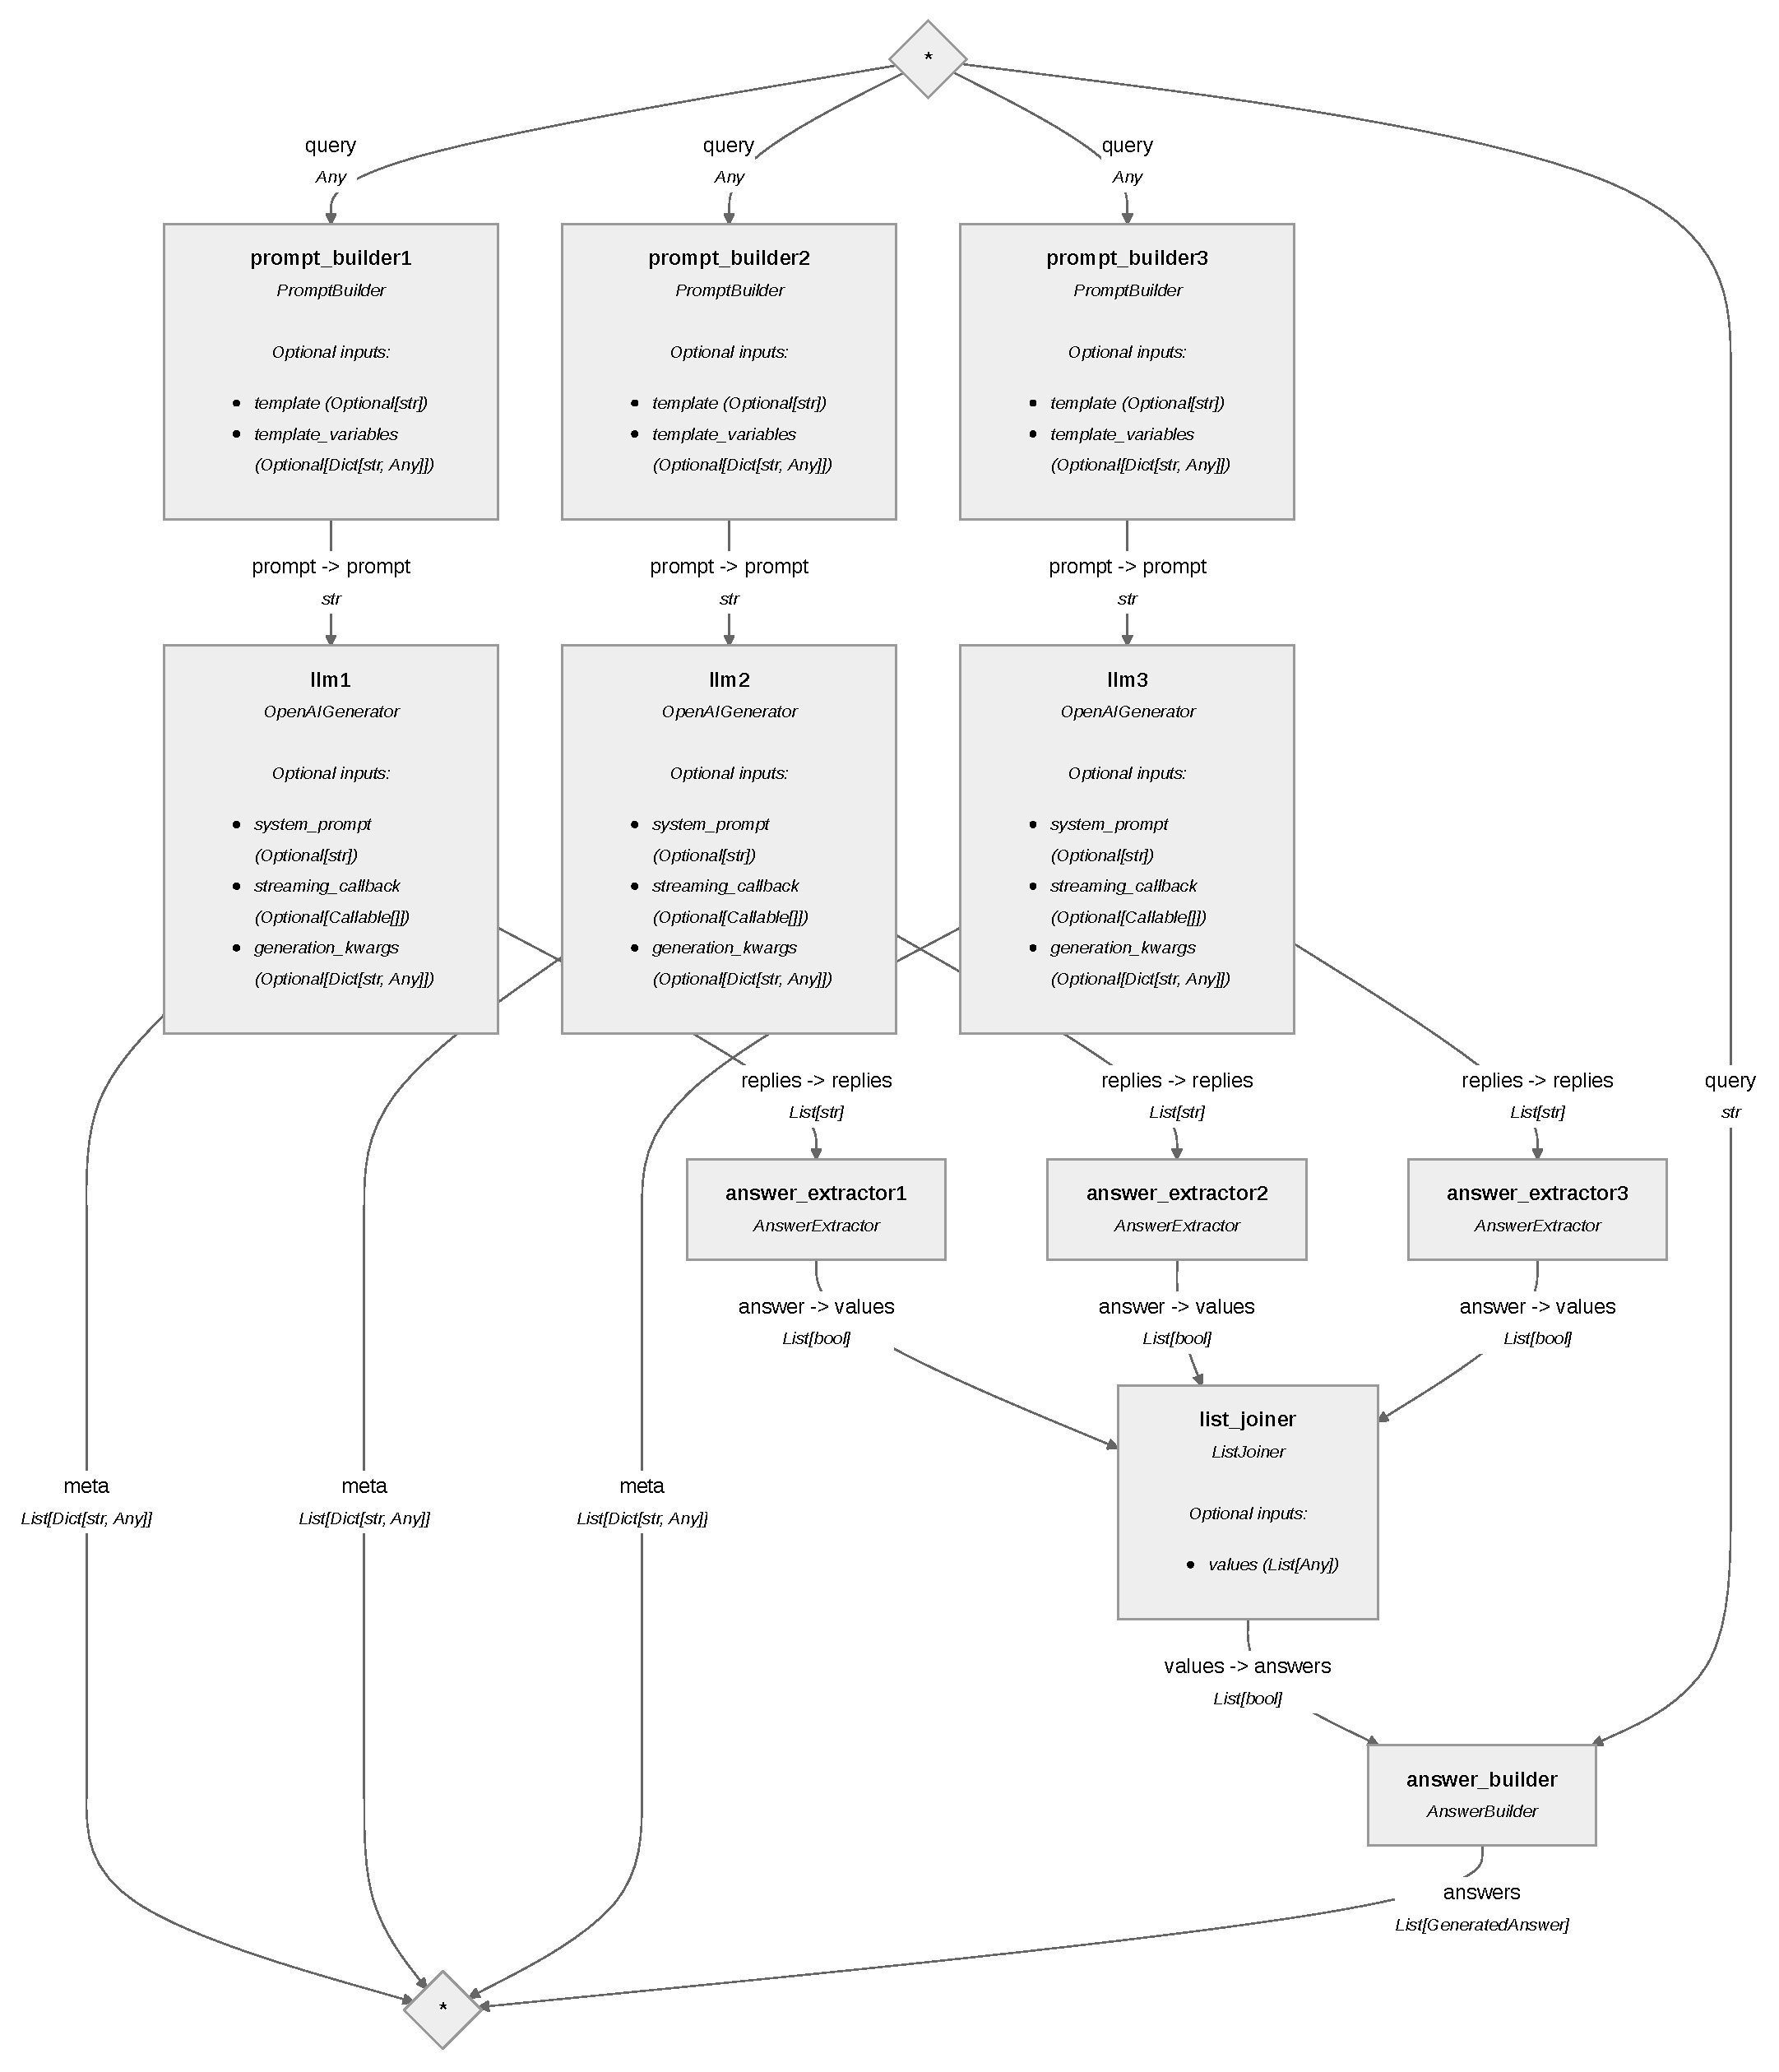
\includegraphics[width=0.95\textwidth]{images/baseline_ciri.pdf}
    \caption{Pipeline diagram of the Ciri baseline implementation}
    \label{fig:pipeline_ciri}
\end{figure}








% Bibliography
% \bibliographystyle{plainnat} % apalike
\bibliographystyle{plain}
\bibliography{literature.bib}    % load file literature.bib

\end{document}
